\pdfminorversion=4
\documentclass[]{article}
\usepackage[utf8]{inputenc}
\usepackage{amssymb,latexsym,amsmath}
\usepackage[a4paper,top=3cm,bottom=2cm,left=3cm,right=3cm,marginparwidth=1.75cm]{geometry}
\usepackage{graphicx}
\usepackage[colorlinks=true, allcolors=blue]{hyperref}
\usepackage{float}

\setlength{\parindent}{10ex}

\title{ECE271 Final Design}
\author{Drew Ortega, Jonathan Alexander, Cole Swanson}
\date{\today}

\begin{document}
\begin{titlepage}
    \begin{center}
        \vspace*{1cm}
 
        \Huge
        \textbf{ECE272 Final Design}
 
        \vspace{0.5cm}
        \LARGE
        Controller Input and VGA
 
        \vspace{1.5cm}
 
        \textbf{Drew Ortega}
        
        \textbf{Cole Swanson}
        
        \textbf{Jonathan Alexander}
 
 		\vspace{0.5cm}
        \today
 
    \end{center}
\end{titlepage}

\newpage
	\tableofcontents
\newpage

\section{Introduction}
This design project is meant to create logic capable of receiving data from three different controller inputs: SNES/NES, IR, and PS/2. Using these inputs, the design will allow for control of two separate player objects that will interact when occupying the same square in a grid. The type of input used will be determined by a two bit mode input. Communication with each controller will be handled by separate decoders, and the data from each controller will be fed into the top level module, and decoded into the desired inputs: up, down, left, and right. The inputs pressed will determine the output displayed through a VGA output, which will consist of a 2x2 grid with squares being empty or filled by a player object, signified by a change in color. The VGA counter and decoder are based on designs from the ECE272 lab course. \\~\\
This design seeks to implement a simple game, two players(differentiated by color) in a grid that can collide with each other. The inputs for each player are handled separately, and ??as a result the input for either player can differ from the other. Specific inputs from each type of controller are mapped to the up, down, left, and right movements, and pressing those buttons, or a combination of them, will result in movement of the player object. If both players are in the same square, the color of that square will be a combination of the two player's colors. 



\section{Top Level Design}
\begin{figure}[H]\centering
    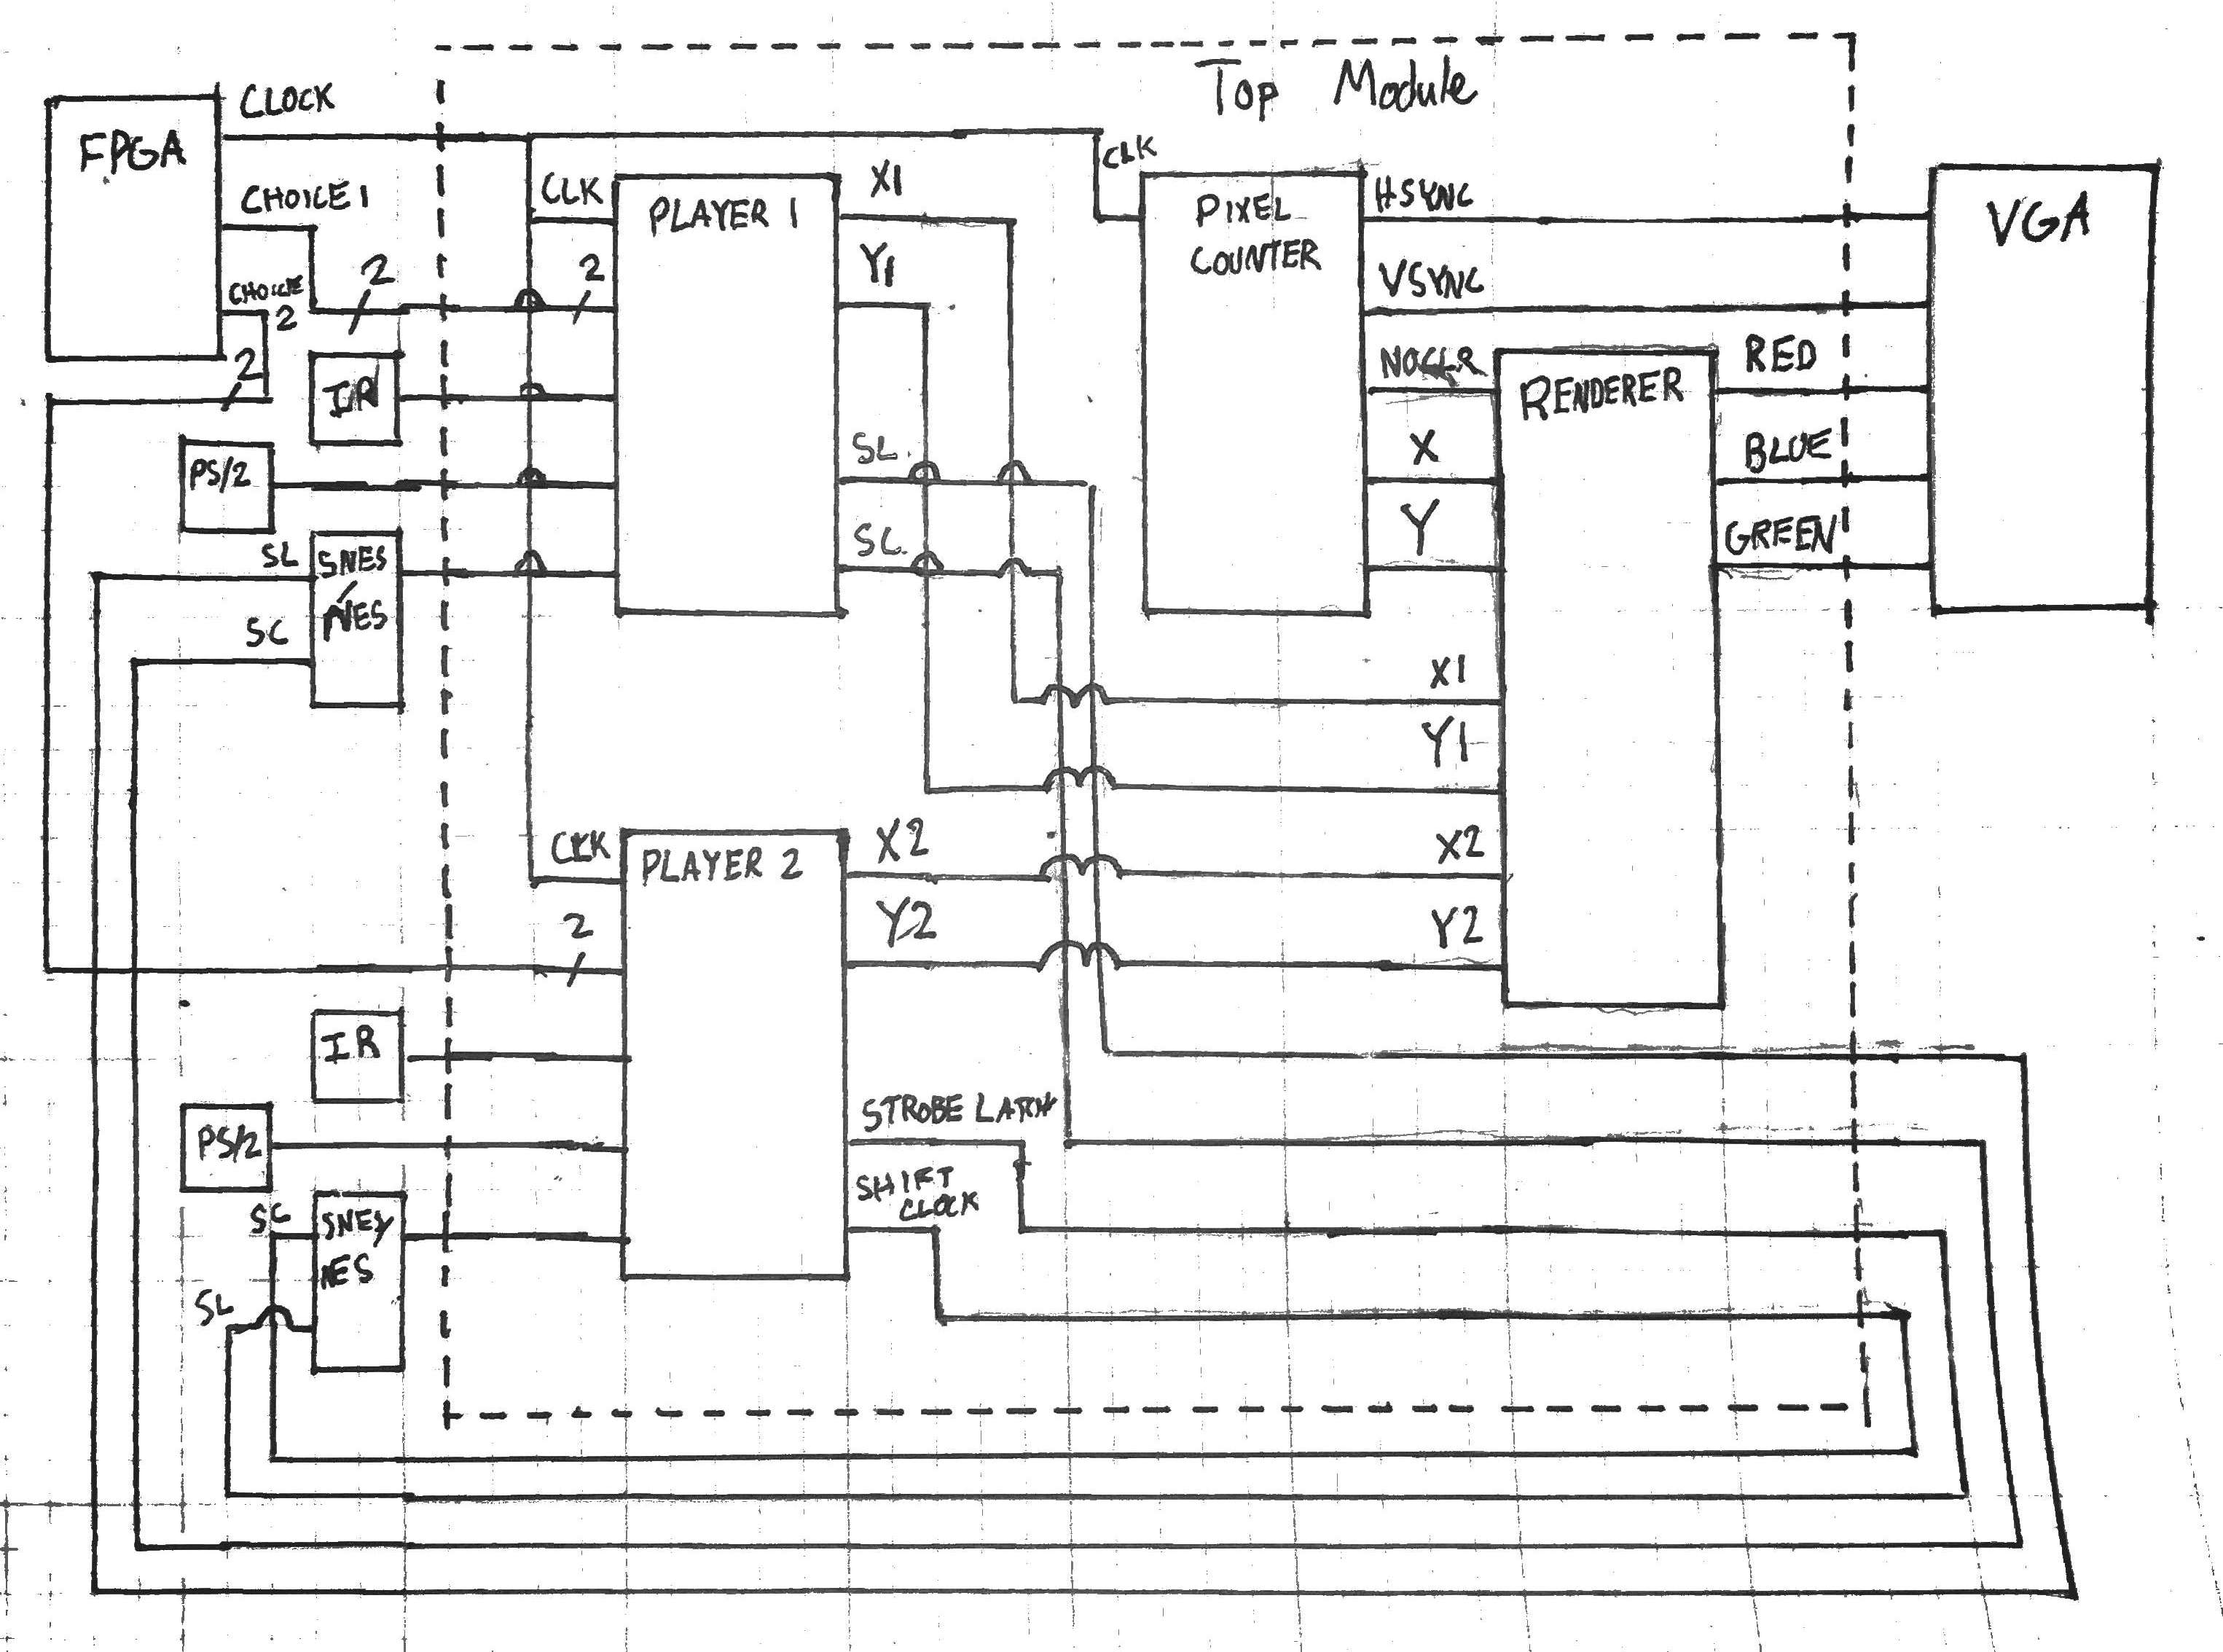
\includegraphics[width=\linewidth]{figures/Top_Block.jpg}
    \caption{Top Level Design Block Diagram} 
    \label{fig:TopLevelDesign}
\end{figure}
TODO

\section{Video Output}\
\label{vidoutput}
TODO

\section{Controllers}
\subsection{NES/SNES Controller}
The NES and SNES controllers utilize three lines to transfer data, along with a ground and 5V power supply. Communication wit the controllers uses a data latch line, clock line and data line. The clock and data latch lines are supplied to the controller, while the data line is generated. When the latch line is driven high, the controllers log the pressed buttons within an active low shift register. The first bit of this register is automatically output on the data line. Whenever the clock input is cycled, the shift register moves along by one bit. The NES controller has eight buttons, and an eight bit shift register, while the SNES has sixteen buttons and a sixteen bit shift register. The data latch can then be cycled to obtain a new set of inputs. For this design, the up, down, left, and right inputs were of interest. Within the NES controller, the zeroth bit of the shift register corresponds to the right input, the first to  the left input, the second to the down input, and the fourth to the up input. The final four inputs were ignored. Within the SNES controller, the up input corresponds to the fifth bit in the shift register, the down input to the sixth bit, the left input to the seventh bit, and the right input to the eight bit. \\~\\
To communicate with the NES or SNES controllers, the host must do the following:
\newline
1. Drive the data latch input high to populate the shift register
\newline
2. The first data bit can now be read
\newline
3. The clock input should be driven high, then low
\newline
4. The next data bit can now be read
\newline
5. Steps 3-4 should be repeated 7 times for the NES, 15 times for the SNES(as the first bit of the register is already present, one less clock cycle is needed)
\subsection{IR Controller}
\subsubsection{Self-Clocking Signal}
\begin{figure}[H]\centering
    
\includegraphics[width=0.5\linewidth]{figures/placeholder.png}
    \caption{Manchester Code/Bi-Phase Coding: from Data to Output} 
    \label{fig:biPhaseExample}
\end{figure}
\label{subsubsec:selfClockingSignal}
The IR Controller uses a self-clocking signal to send data to the receiver.
For a signal to be self-clocking, the source must have a clock of a specified speed and a serial data output.
The source combines the clock and serial output in to a single serial output of a designated encoding.
For the IR Controller, the IEEE Manchester Code specification, also known as "Bi-Phase Coding" (BPC), is used.
For BPC, the source checks the data it wishes to output on every rising edge of its clock.
If the data to be transmitted is a 1, than the serial output is driven to mimic the clock for that cycle.
Essentially, it rises on a rising edge of a clock, and falls on the falling edge of the clock.
If the data to be transmitted is a 0, than the serial output begins to be the inverted signal of the clock.
It falls on the rising edfe of the clock, and rises on the falling edge of the clock. 
What a Bi-Phase Coding might look like can be found in Figure \ref{fig:biPhaseExample}.
\subsubsection{IR Signal \& RC 5 Code}
\begin{figure}[H]\centering
    
\includegraphics[width=0.5\linewidth]{figures/placeholder.png}
    \caption{RC 5 Code - Chunk and delay}
    \label{fig:rc5Code}
\end{figure}
This implementation of IR reception assumes that the IR signal received will be in the form of BPC, as explained in \ref{subsubsec:selfClockingSignal}.
There are several standards for IR data transmission. The that is decoded for this design is the RC 5 Code (RC5).
RC5 sends data in chunks, separated by a static amount of clock cycles at 36 kHz. Each chunk is has four sections, totalling to 14 bits.
\begin{itemize}
    \item[-] Section 1 - Start Bits (2 bits): Help orient the reciever to understand source clock timing.
    \item[-] Section 2 - Toggle Bit (1 bit): Defines whether or not this chunk is a new key press or a held key already transmitted.
    \item[-] Section 3 - Address (5 bits): Defines the address of the receiver. If this does not match the expected address, the data is ignored.
    \item[-] Section 4 - Data (6 bits): Defines the actual data of the chunk, up to 6 bits. A single combination represents an individual button.
\end{itemize}
After the full chunk has been transmitted, the serial data signal is driven to 0 for 50 clock cycles before data is transmitted again.
After the 50 clock cycles, if a button on the controller is still being pressed, the transmitter on the controller will send the same data chunk again, except the toggle bit will be 0 instead of 1.
If after 50 cycles no data is read, there is no button being pressed or the receiver is not receiving data.\cite{vishayIr}
The structure and timing of RC 5 Code can be found in Figure \ref{fig:rc5Code}.
\subsection{PS/2 Controller}
The standard for PS/2 has multiple possible states for the peripheral device.  It can be in its idle state, a communication halt state, and a host-to-device state.
For this projects' purposes, we will only implement the idle state, as it is the default state, where the device sends key press and unpress updates to the host.
The idle state's standard functions almost exactly like a Serial Peripheral Interface.  The negative edge of the clock signal driven by the device indicates the data value for each bit.
There is a standard for what each bit in the 11 bit sequence represents.  The sequence is as follows:
\begin{itemize}
    \item[-] 1 start bit - This is always 0
    \item[-] 8 data bits - Least significant bit first
    \item[-] 1 parity bit - Odd parity
    \item[-] 1 stop bit - This is always 1
\end{itemize}
The 8 data bits are a unique number that represents a specific key being pressed, or unpressed.  The parity bit is a bit representing how many 1s there are in the data bit.  It functions as a quick and simple error check, if the parity bit does not match the data then you know the data was corrupted somehow.

\section{HDL Modules}
\subsection{NES/SNES input decoder}
\begin{figure}[H]\centering
	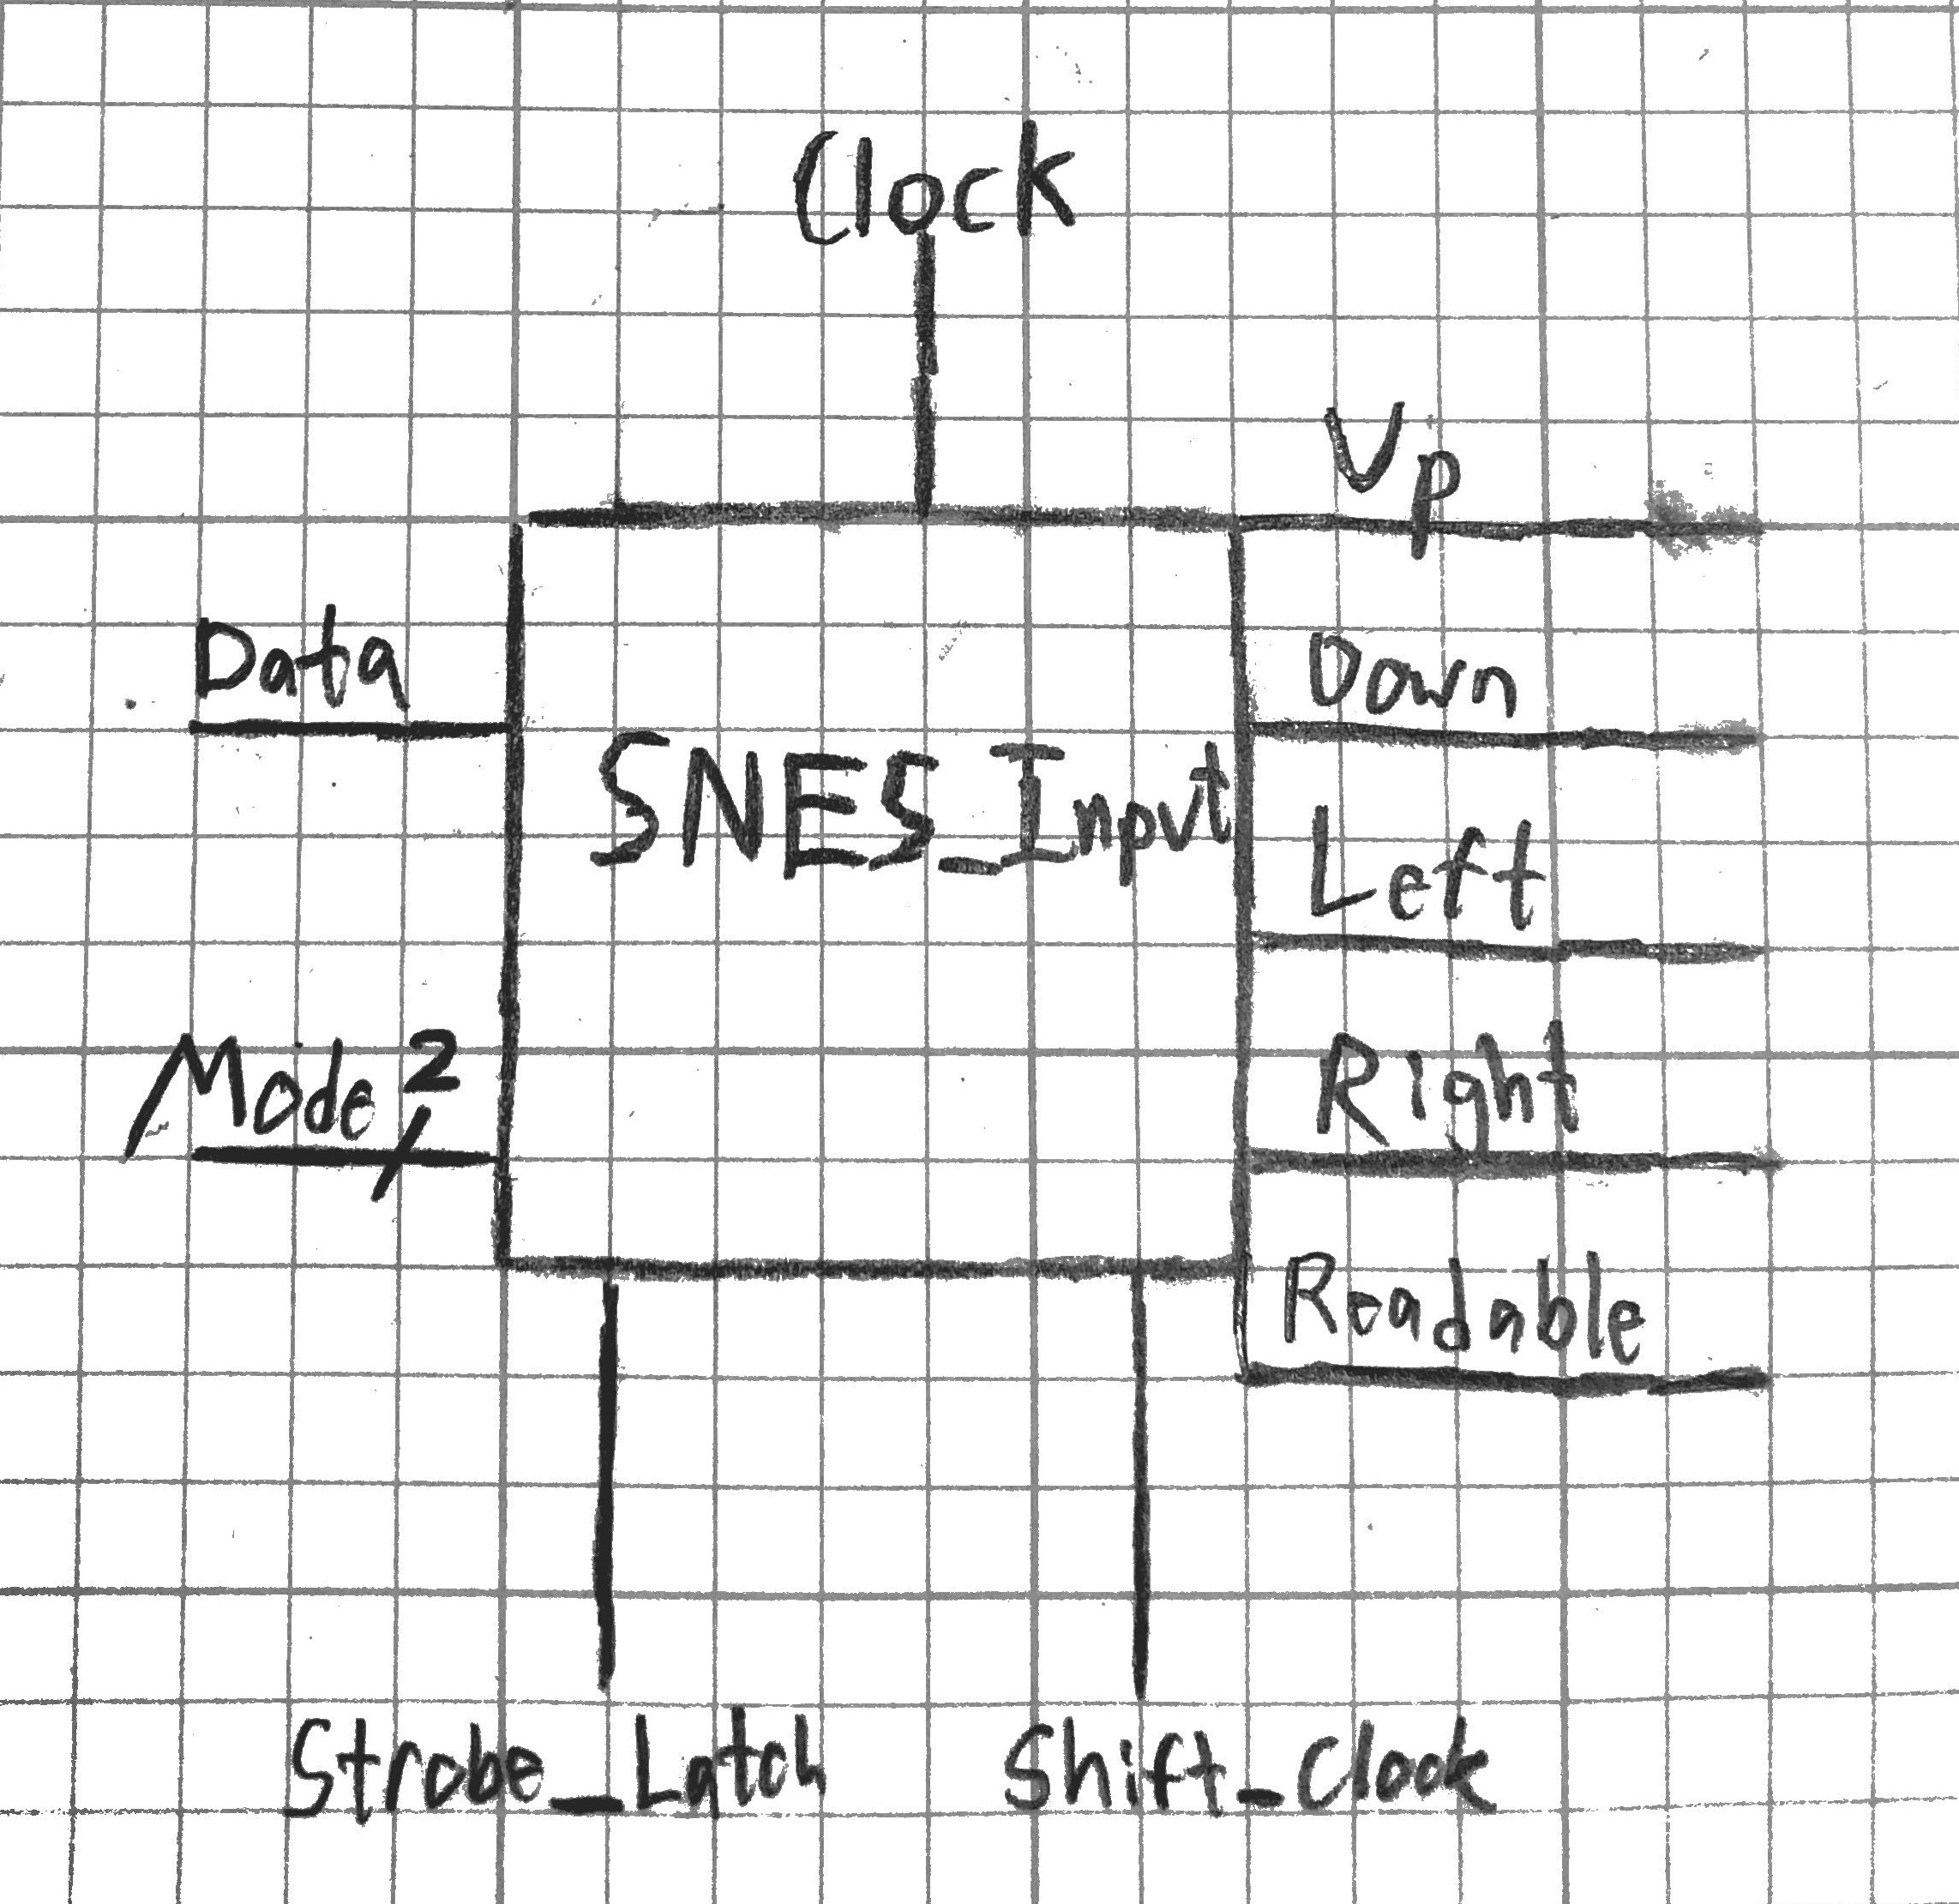
\includegraphics[width=\linewidth]{figures/SNES_Input_Diagram}
	\caption{Block Diagram of the NES/SNES input decoder}
\end{figure}
\begin{figure}[H]\centering
	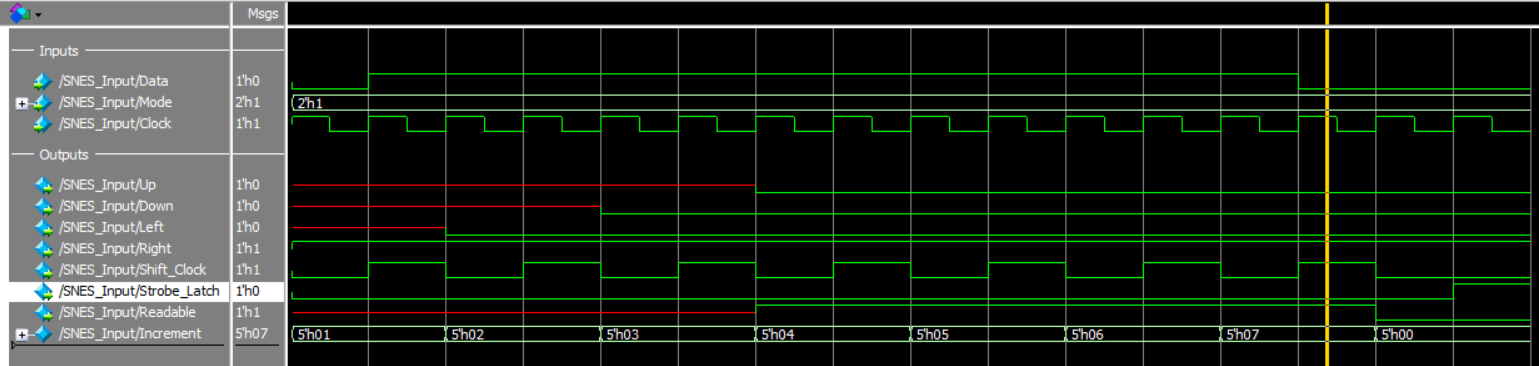
\includegraphics[width=\linewidth]{figures/NES_Input_Sim.png}
	\caption{ModelSim of the NES/SNES controller decoder in NES mode.}
\end{figure}

\begin{figure}[H]\centering
	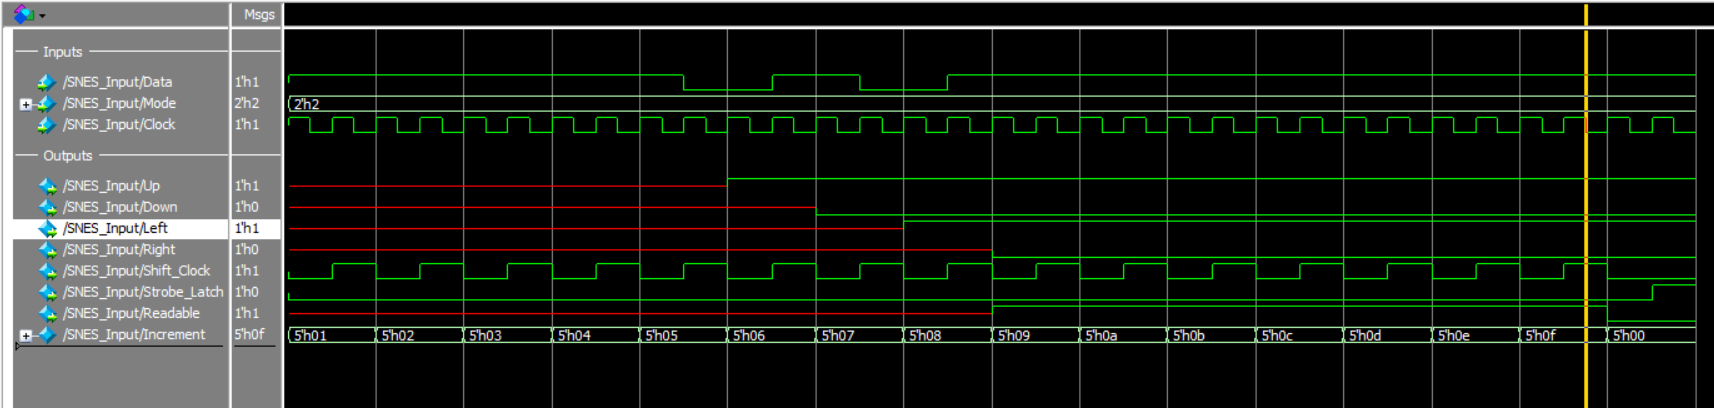
\includegraphics[width=\linewidth]{figures/SNES_Input_ModelSim.png}
	\caption{ModelSim of the NES/SNES controller decoder in SNES mode}
\end{figure}
Inputs: One bit data representing the current bit from the controller shift register, one bit clock, and two bit mode used to determine which controller is in use(NES or SNES)\\~\\
Outputs: One bit up, down, left, and right representing the decoded values from the controller, and one bit readable output which is driven high once the current set of values have been decoded. Also present are the one bit strobe latch output, which functions as the data latch for the controller to be driven high then low to log the inputs to the controller, and a one bit shift clock, which is used to shift the values in the controller shift register. \\~\\
Simulations: \\~\\
NES: \\
For this simulation, the data bit for right was driven low(representing an input of 'right'). The data\_latch is initially driven high. As expected, the decoder logs the right input as pressed, and continues through the inputs by providing a shift\_clock to the controller. Once the data has been cycled three times, all values of interest are accounted for, and the readable output is driven high. After seven cycles of the output, the data\_latch is again driven high and readable is driven low; new inputs are ready to be read. The value of increment represents the current bit of the shift register.\\~\\
SNES: \\
For this simulation, the data bits for up and left were driven low(representing inputs of 'left' and 'up'). The data\_latch is initially driven high. As expected, the decoder logs the up and left inputs as pressed, and continues through the inputs by providing a shift\_clock to the controller. Once the data has been cycled eight times, all values of interest are accounted for, and the readable output is driven high. After fifteen cycles of the output, the data\_latch is again driven high and readable is driven low; new inputs are ready to be read. The value of increment represents the current bit of the shift register.\\~\\
This module will use the system clock to drive its logic. On the first clock cycle, the data latch output will be driven high to log the controller inputs. The data latch will then be driven low, and the shift clock will be cycled seven times for the NES controller, or fifteen times for the SNES controller, with the bit corresponding to the inputs of interest recorded. Once all inputs of interest have been recorded, the readable output will be driven high, signaling all inputs are accounted for. Pressed buttons on the controllers will be signaled by a high value on the corresponding output from the decoder(up, down, left, or right). 

\subsection{IR Input Top Module}
\begin{figure}[H]\centering
    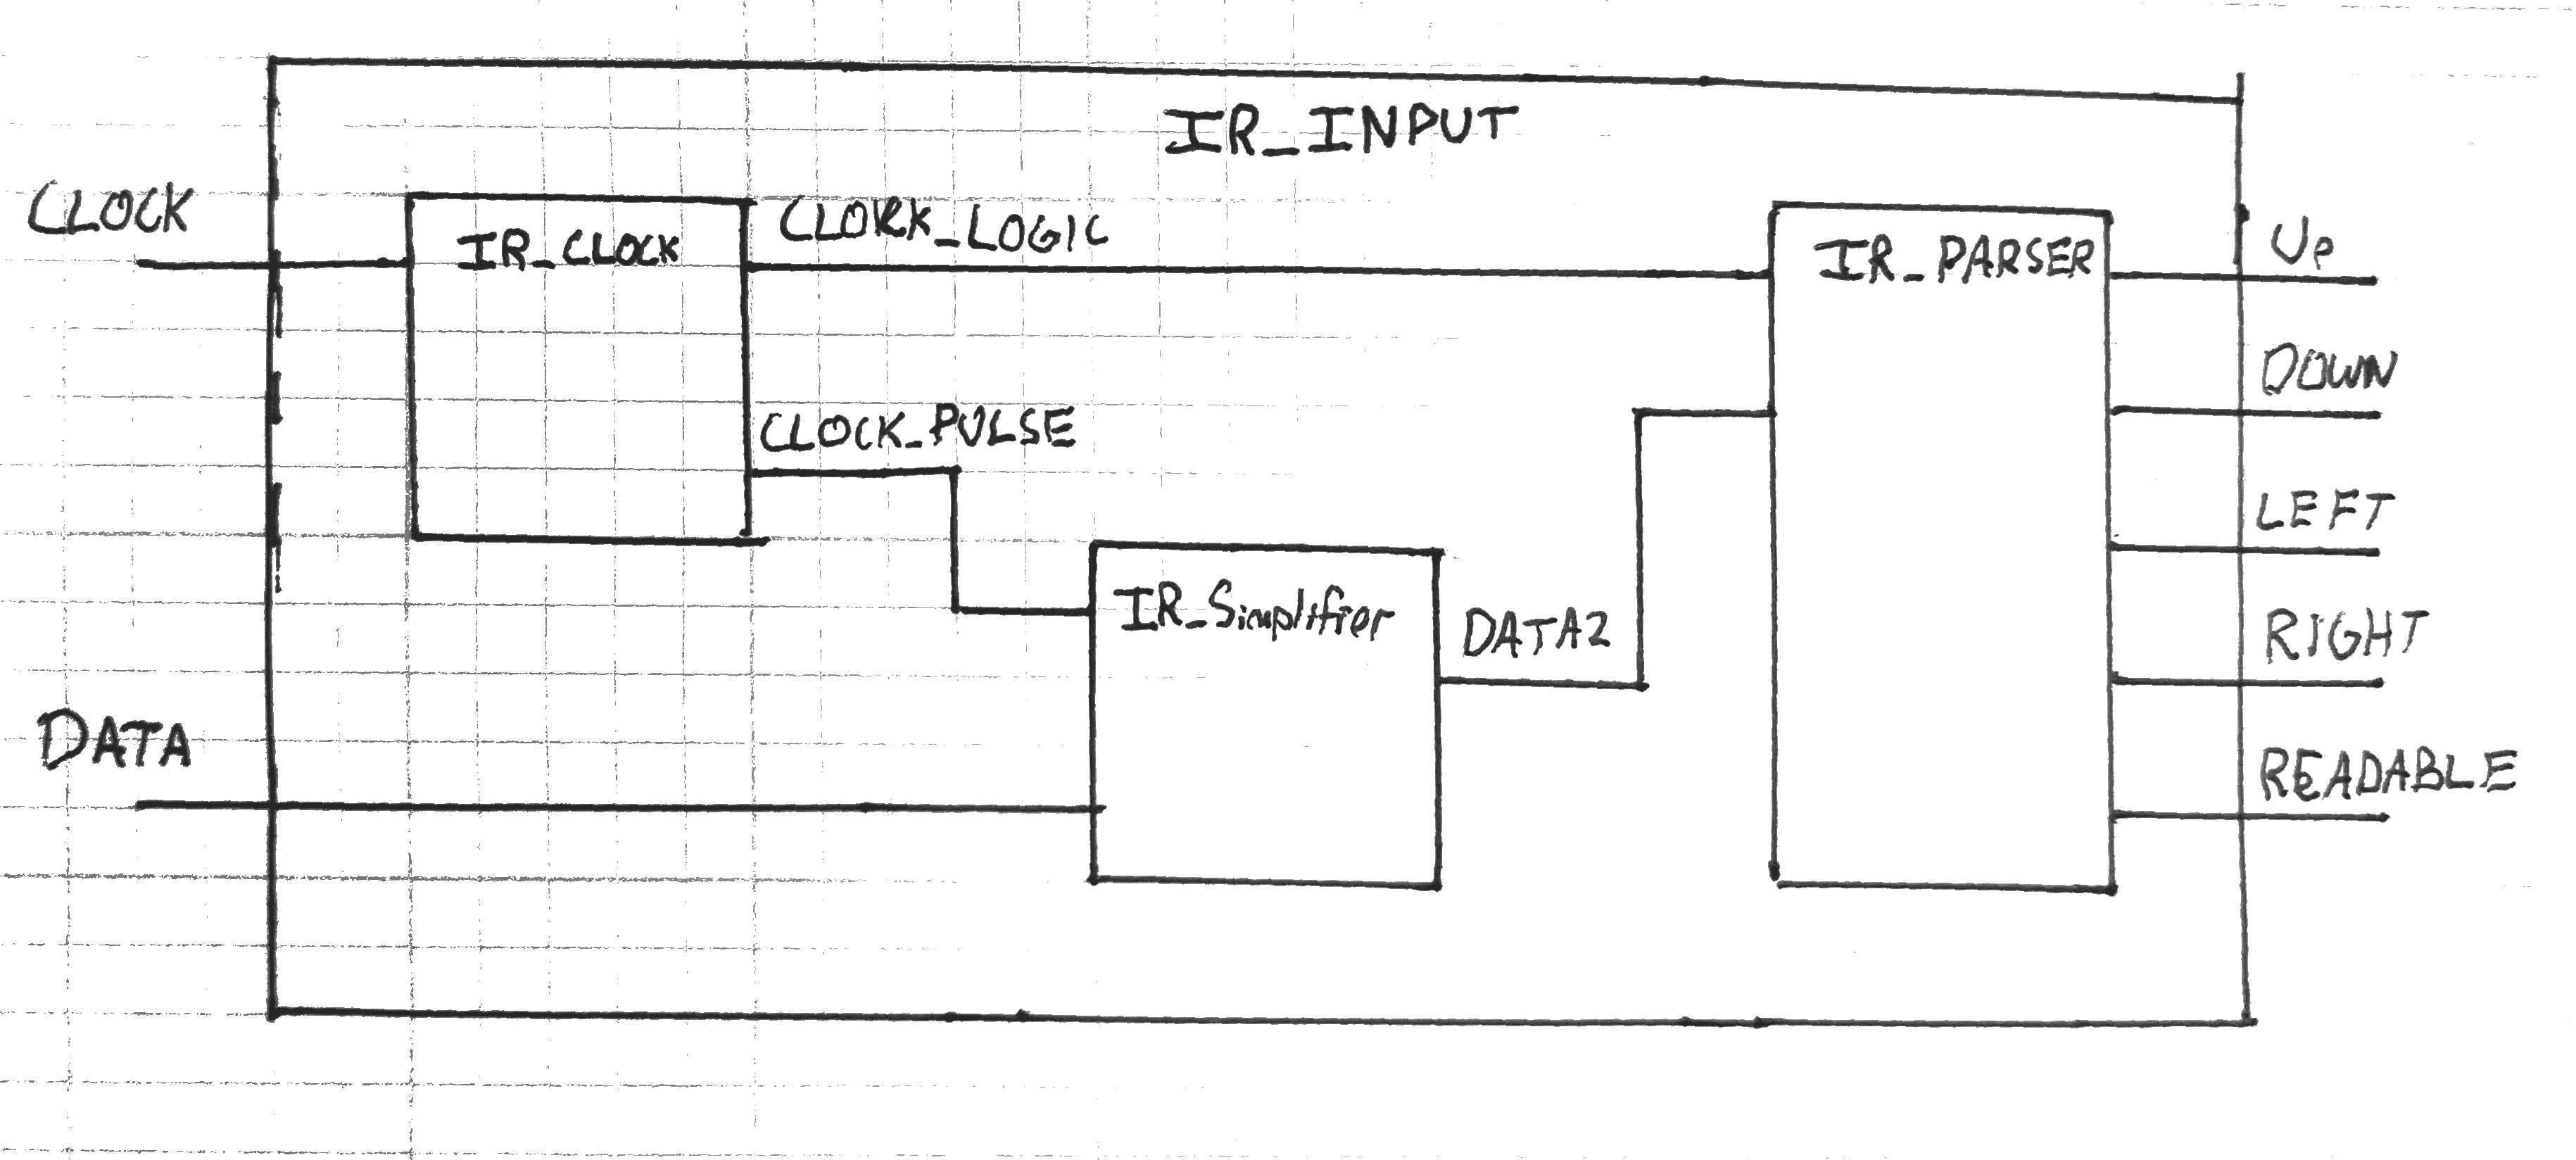
\includegraphics[width=\linewidth]{figures/IR_Input_Block.jpg}
    \caption{IR Top Module Diagram}
    \label{fig:irInputDecoderBlock}
\end{figure}
\begin{figure}[H]\centering
    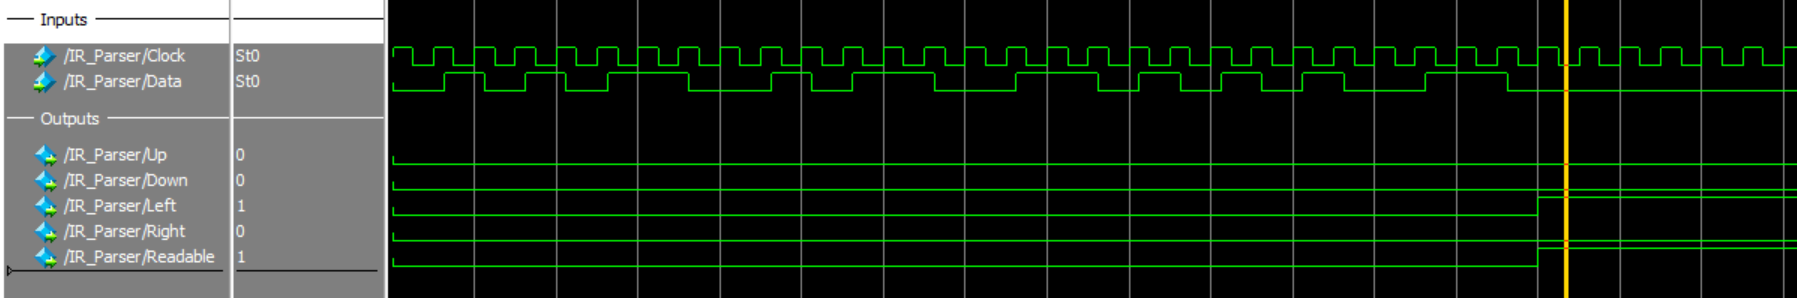
\includegraphics[width=\linewidth]{figures/IR_Input_Sim.PNG}
    \caption{IR Top Module Simulation}
    \label{fig:irInputDecoderSim}
\end{figure}
\paragraph{Input:} One Serial Data stream 'Data', Clock signal.
\paragraph{Output:} One output for each cardinal direction (Up, Down, Left, Right), and signal describing whether or not the directions are valid or not, 'Readable'.
\paragraph{Description:} For the IR Decoder, it was noted that its output must match the output of any other input decoder, such as the SNES/NES and PS/2.
Because of this, the Up, Down, Left, Right, and Readable streams were required to be used for this particular module. This particular model 
\paragraph{Simulation:} TODO

\subsubsection{IR Clocks}
\begin{figure}[H]\centering
    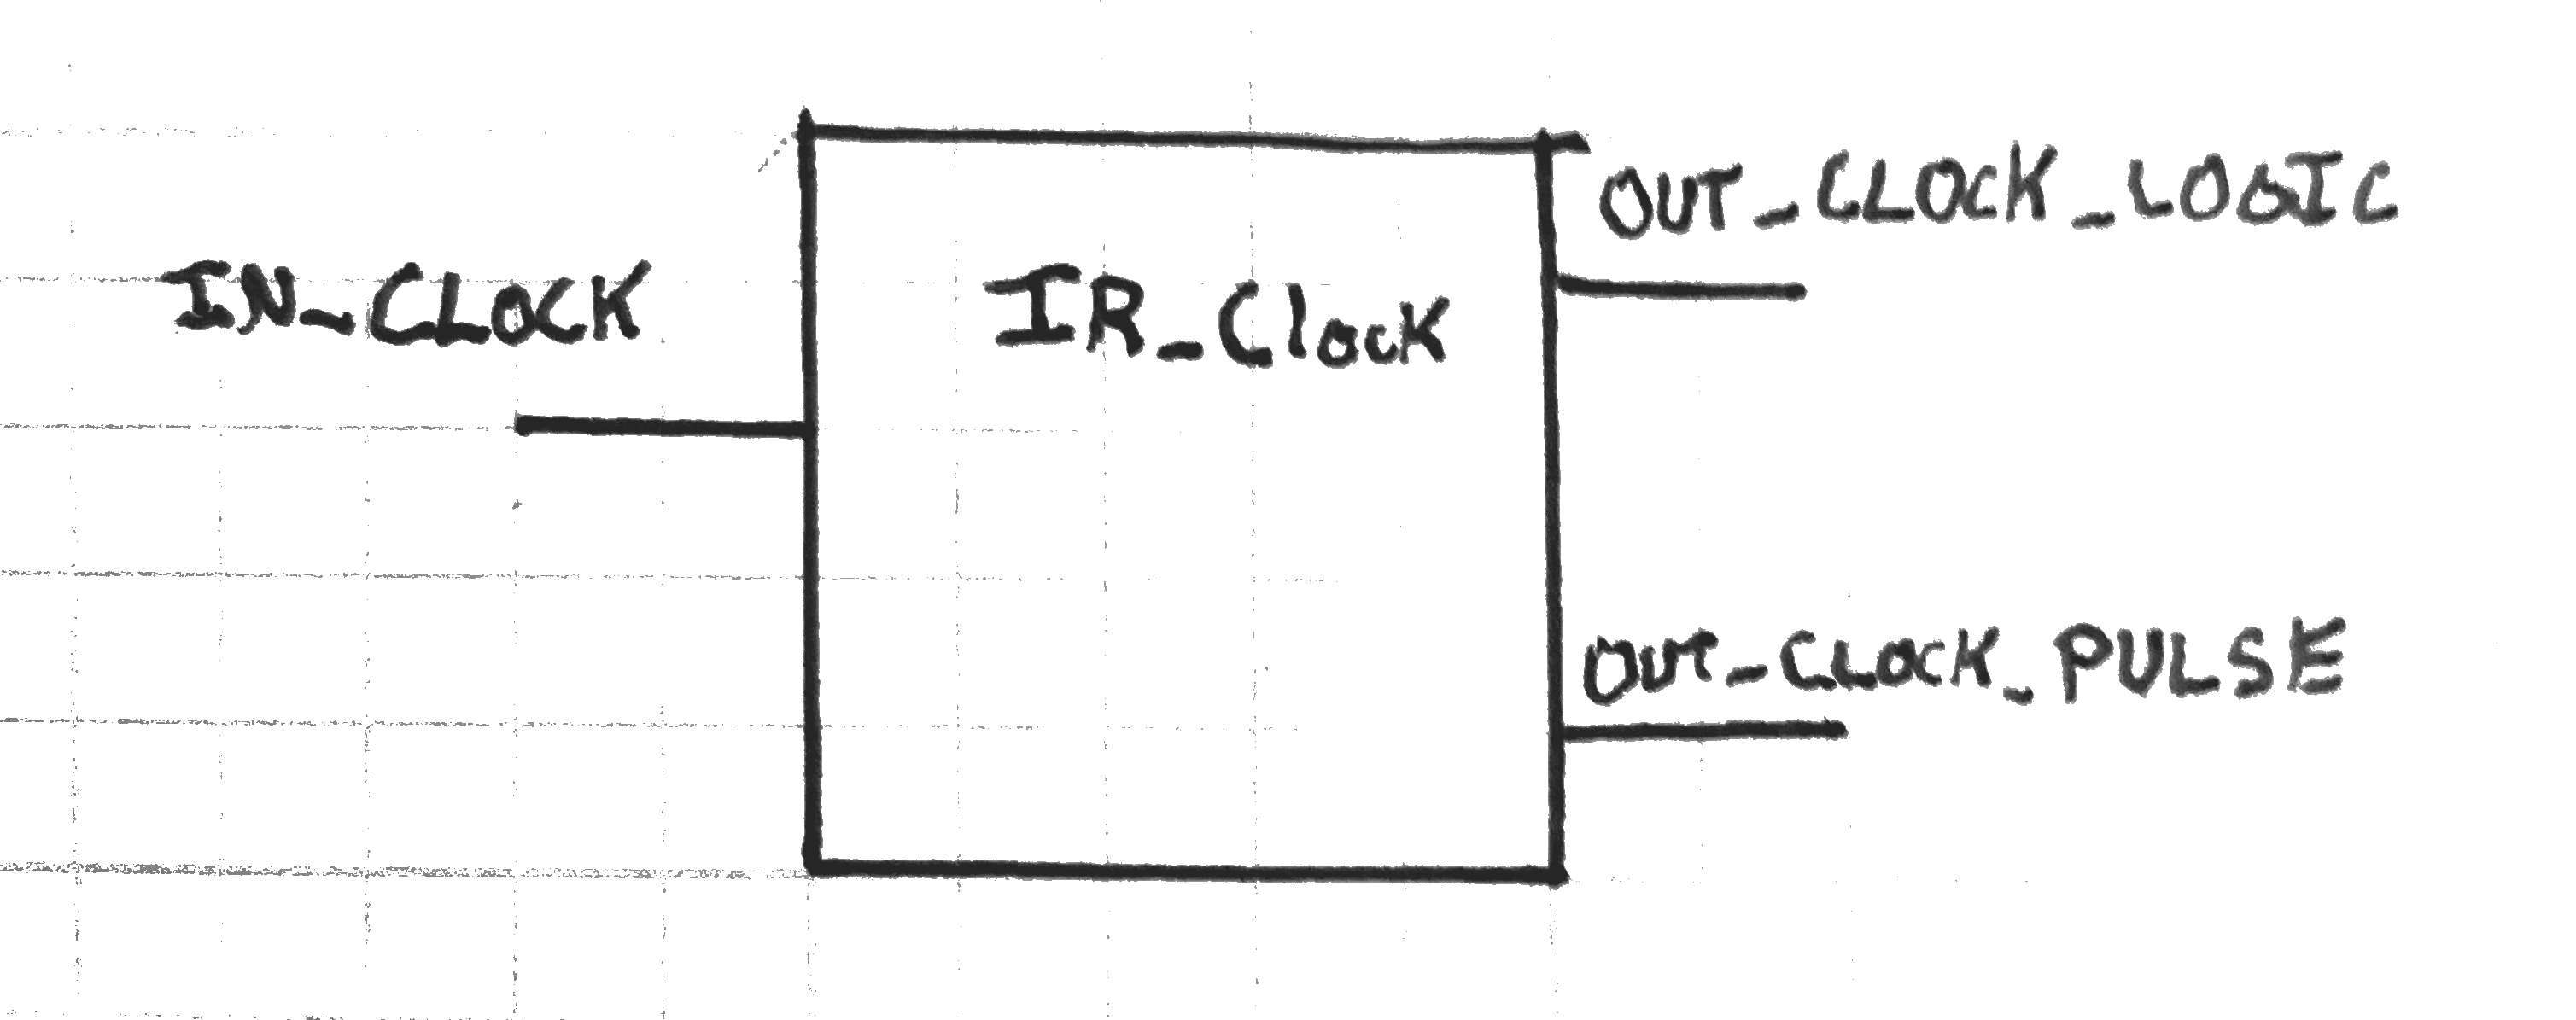
\includegraphics[width=0.9\linewidth]{figures/IR_Clock_Block.jpg}
    \caption{IR Clock Slowing Block Diagram}
    \label{fig:irClockBlock}
\end{figure}
\begin{figure}[H]\centering
    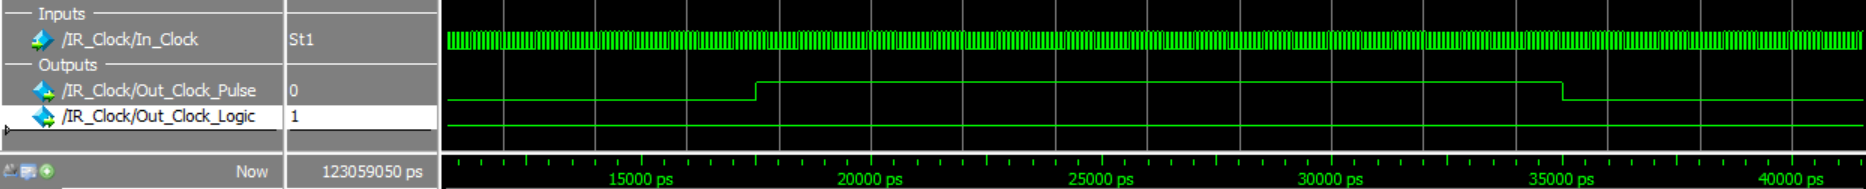
\includegraphics[width=\linewidth]{figures/IR_Clock_Sim1}
    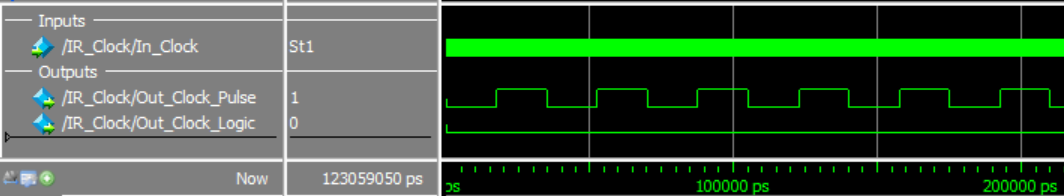
\includegraphics[width=\linewidth]{figures/IR_Clock_Sim2}
    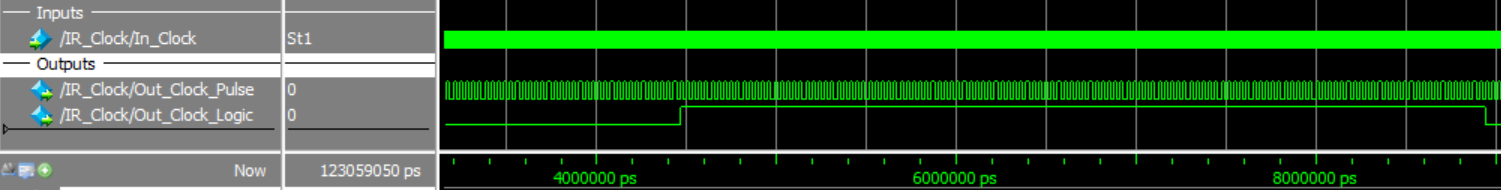
\includegraphics[width=\linewidth]{figures/IR_Clock_Sim3}
    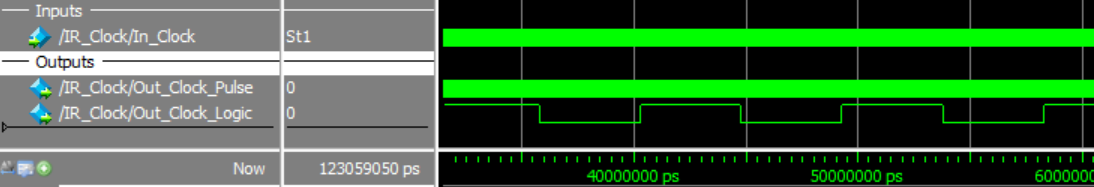
\includegraphics[width=\linewidth]{figures/IR_Clock_Sim4}
    \caption{IR Clock Sim}
    \label{fig:asyncIRData}
\end{figure}
\paragraph{Inputs:} Takes in a single 50 MHz Clock.
\paragraph{Outputs:} Outputs a 
\paragraph{Simulation:} TODO 
\paragraph{Description:} The IR Input reciever takes in the BPC serial data stream and a 50MHz Clock signal. A slowed clock is generated to slow it down to approximately 72 kHz.
This is achieved by dividing the 50 MHz clock by 694. However, if the Clock was flipped every 694 50 MHz cycles, it would have a clock cycle of 36 kHz. 
To account for this, we must double the resulting clock, by dividing the original clock by 347.
With the 72 kHz clock, for each rising edge of this clock the IR signal will have either a rising edge or a falling edge. 
Since the IR signal is asynchronous, meaning its clock will not line up with our clock, the 72 kHz clock can check on each of its rising edges whether or not the Data input is a 0 or a 1.
An example of what the async data vs our internal clock can be found in Figure \ref{fig:asyncIRData}.

\subsubsection{IR Simplifier}
\begin{figure}[H]\centering
    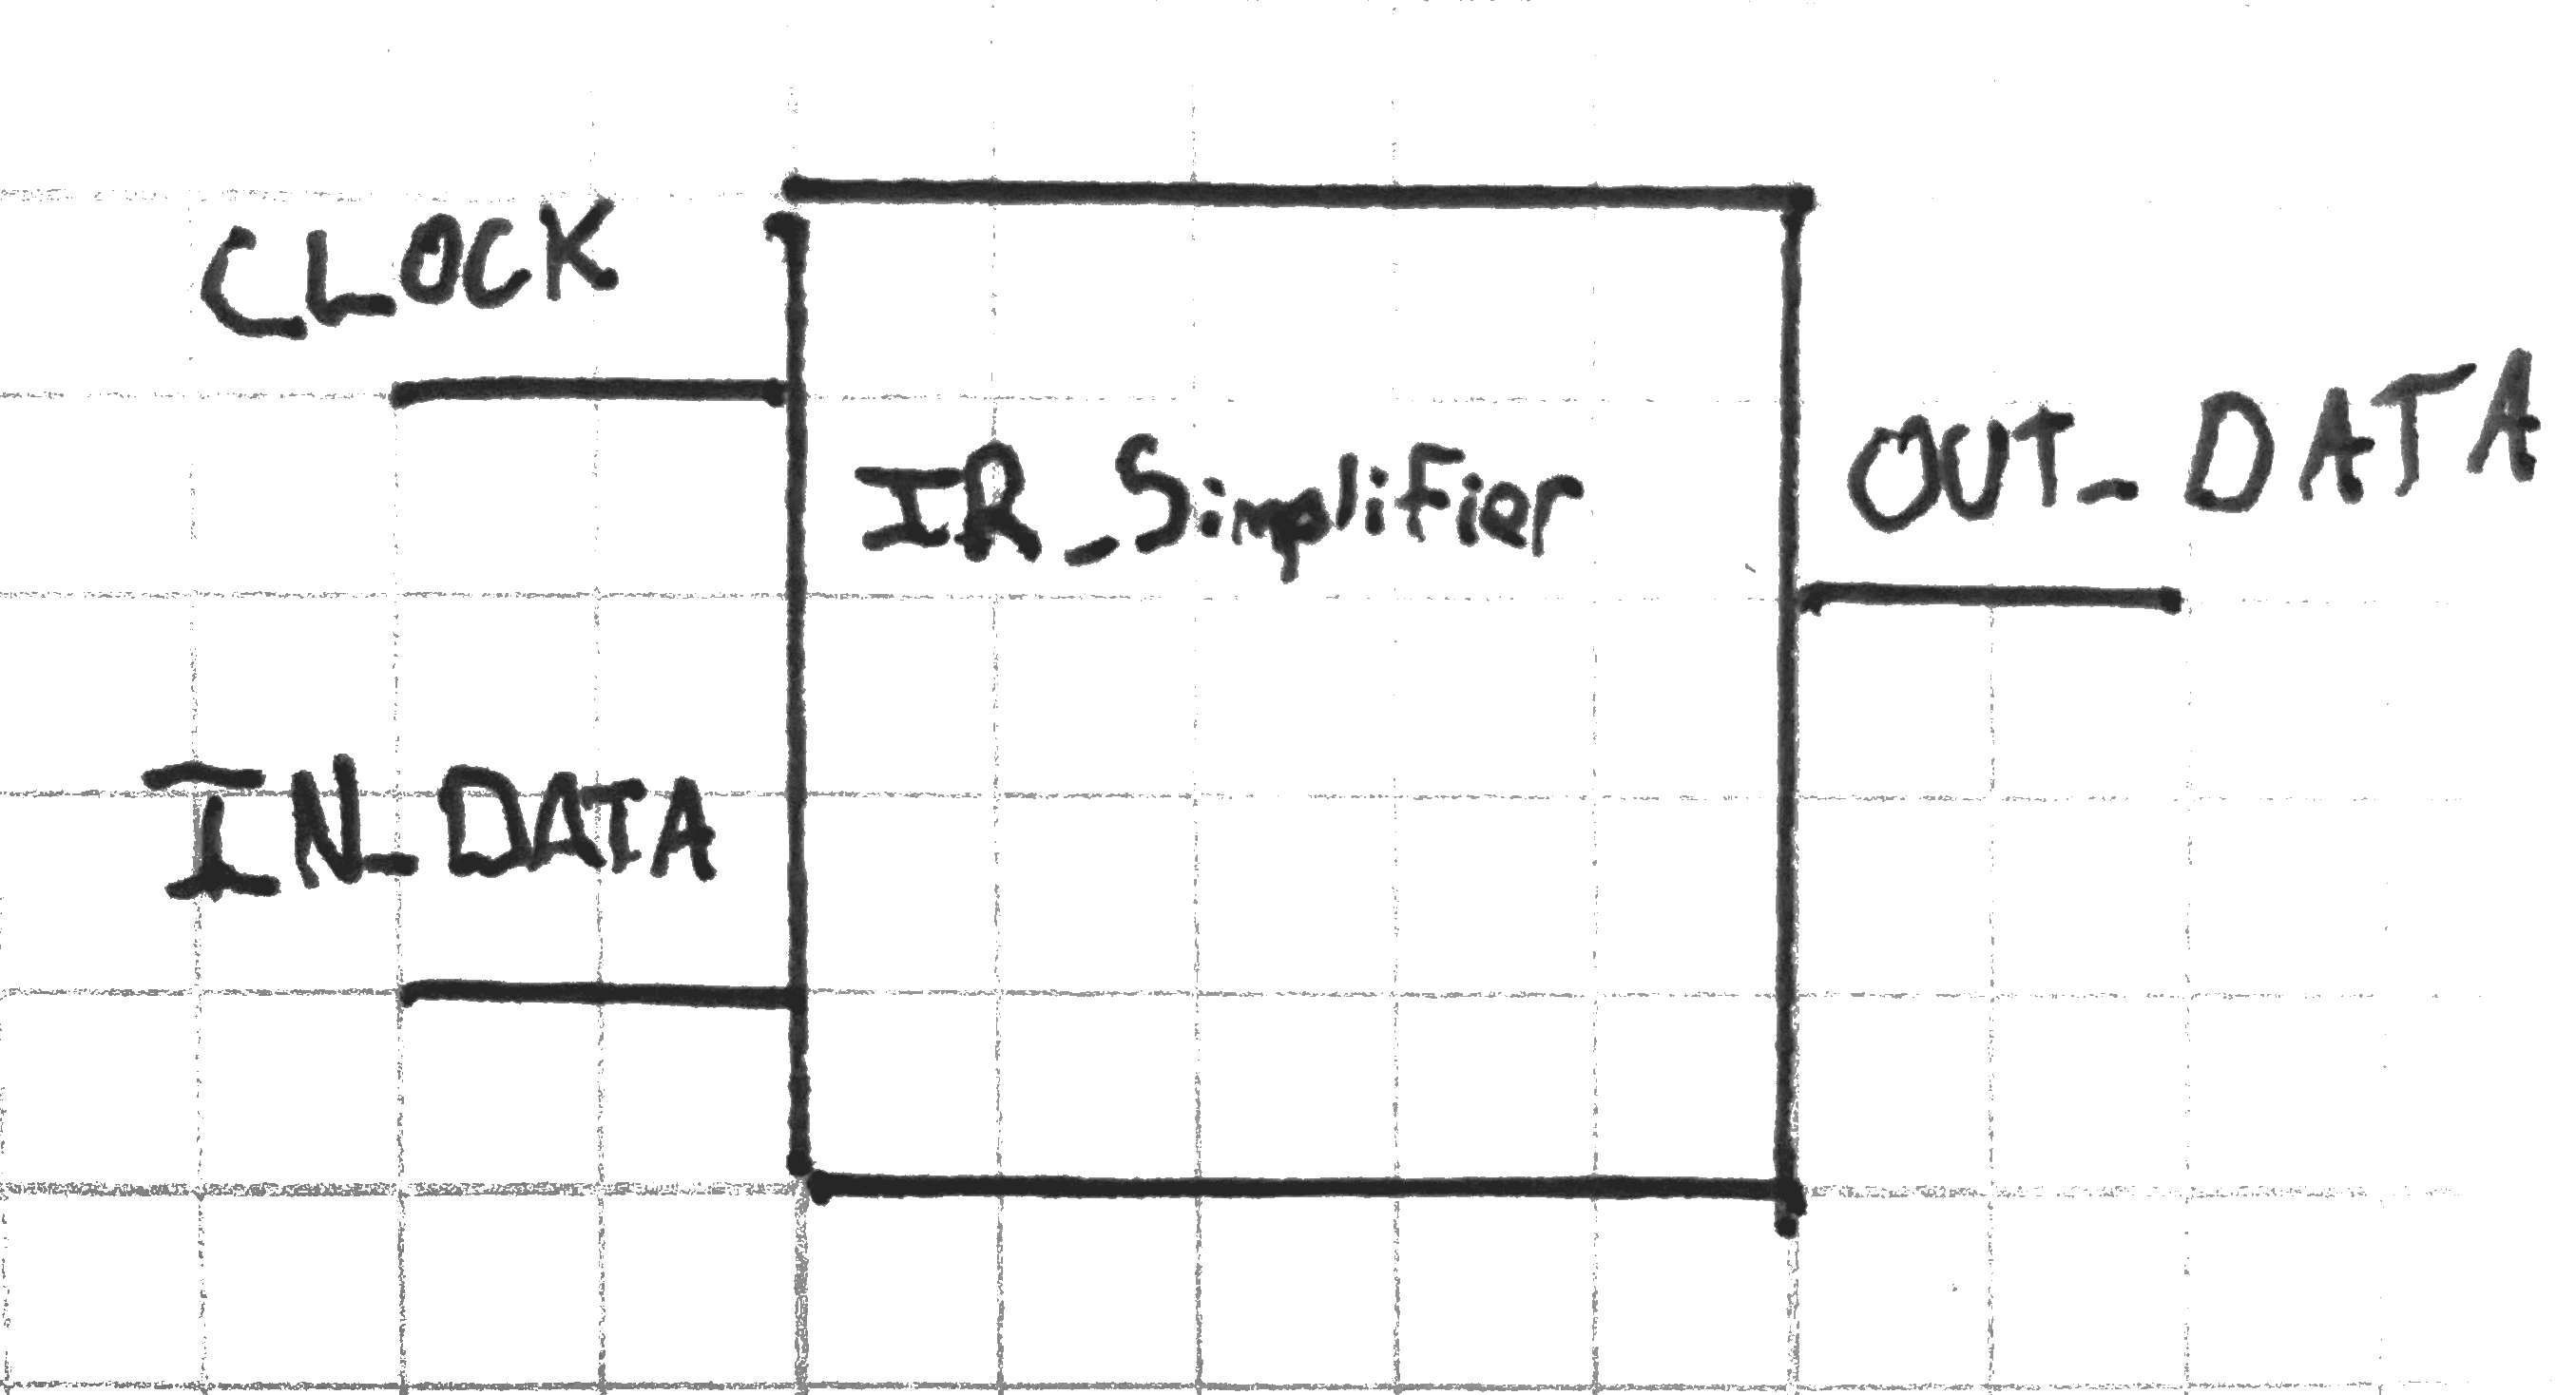
\includegraphics[width=0.6\linewidth]{figures/IR_Simplifier_Block.jpg}
    \caption{IR Simplifier Block Diagram}
    \label{fig:irSimplifierBlock}
\end{figure}
\begin{figure}[H]\centering
    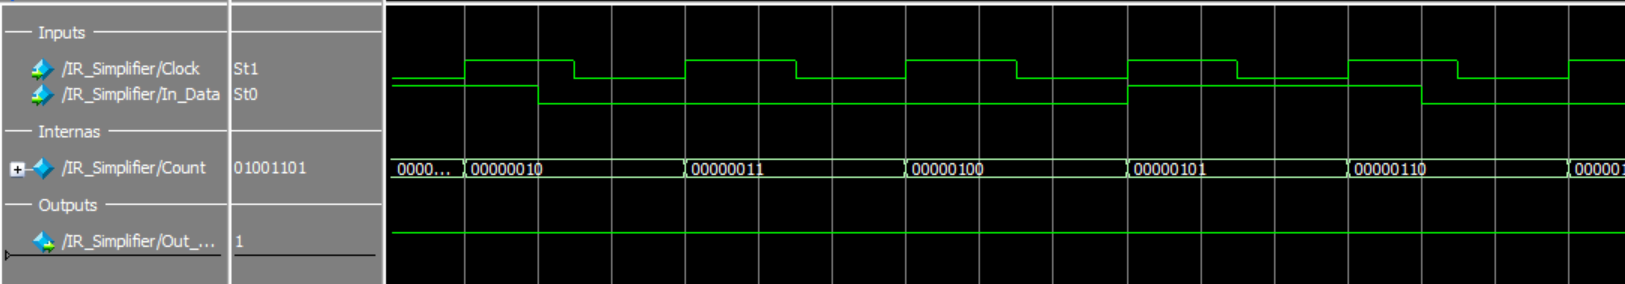
\includegraphics[width=\linewidth]{figures/IR_Simplifier_Sim1.png}
    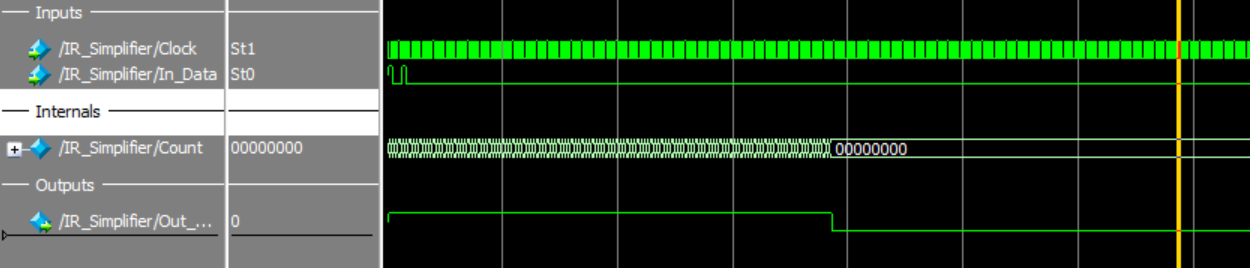
\includegraphics[width=\linewidth]{figures/IR_Simplifier_Sim2.png}
    \caption{IR Simplifier Simulation}
    \label{fig:irSimplifierSim}
\end{figure}
\paragraph{Inputs:} TODO
\paragraph{Outputs:} TODO
\paragraph{Simulation:} TODO
\paragraph{Description:}


\subsubsection{IR Parser}
\begin{figure}[H]\centering
    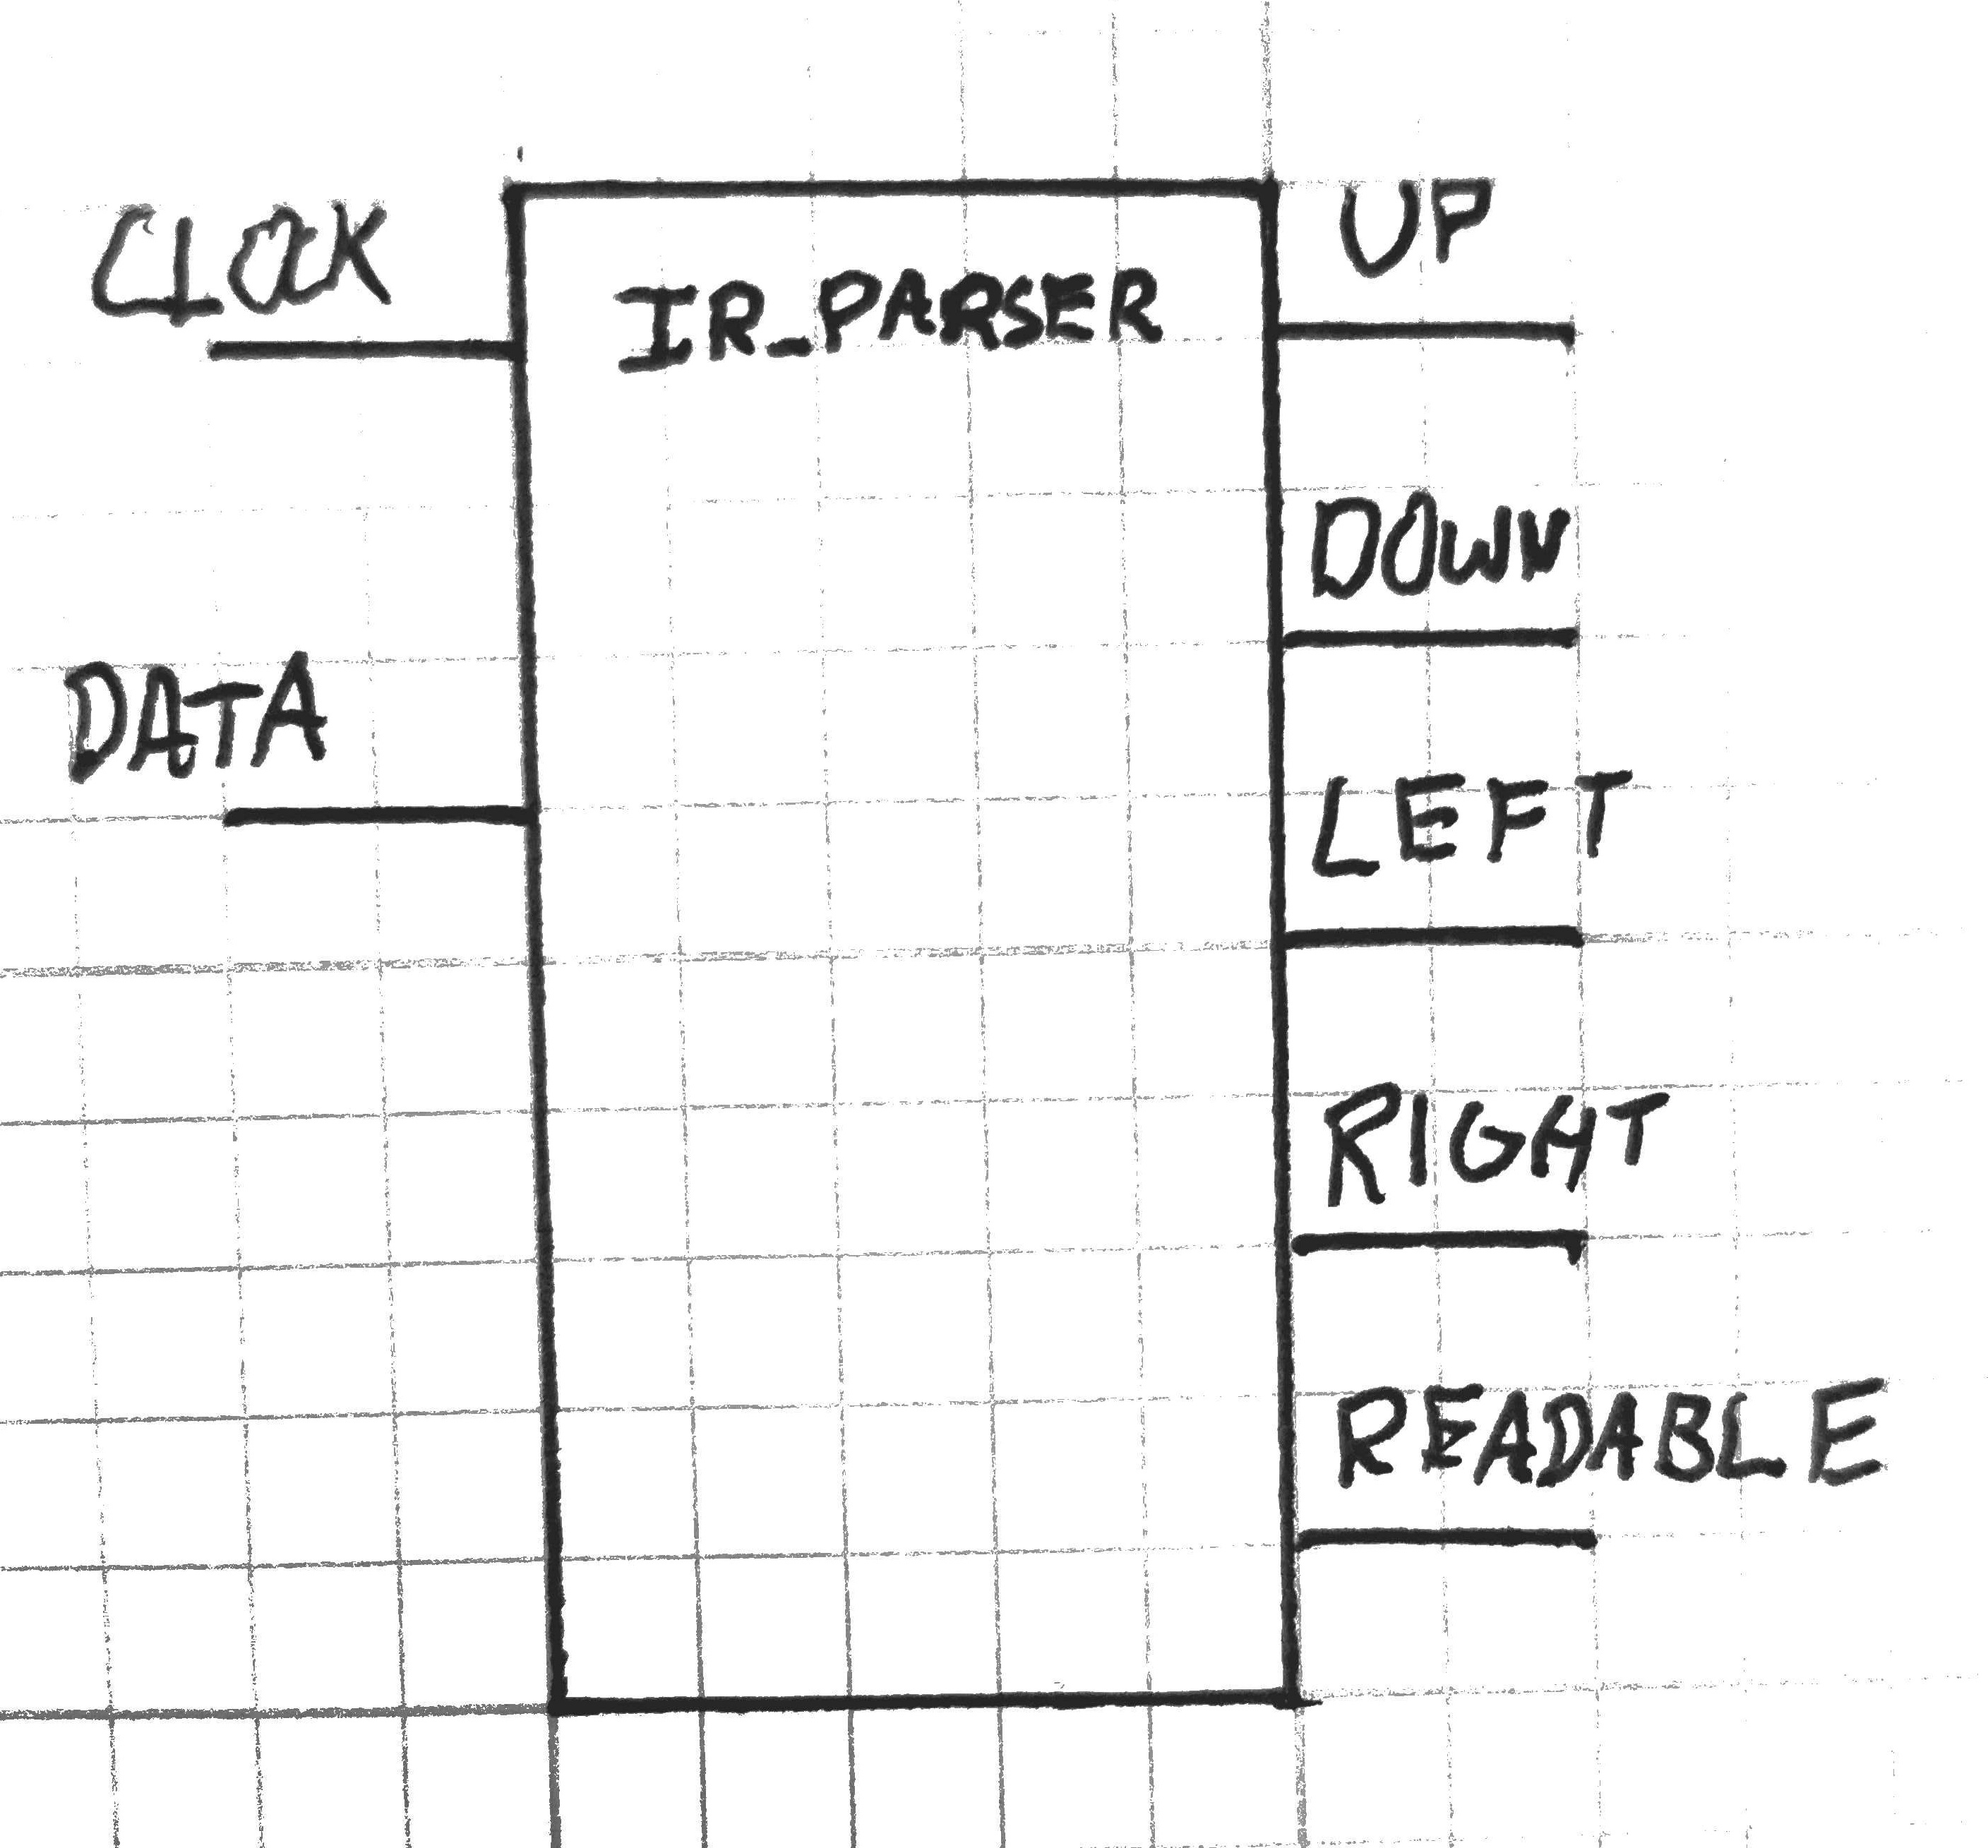
\includegraphics[width=0.5\linewidth]{figures/IR_Parser_Block.jpg}
    \caption{IR Parser Block Diagram}
    \label{fig:irParserBlock}
\end{figure}
\begin{figure}[H]\centering
    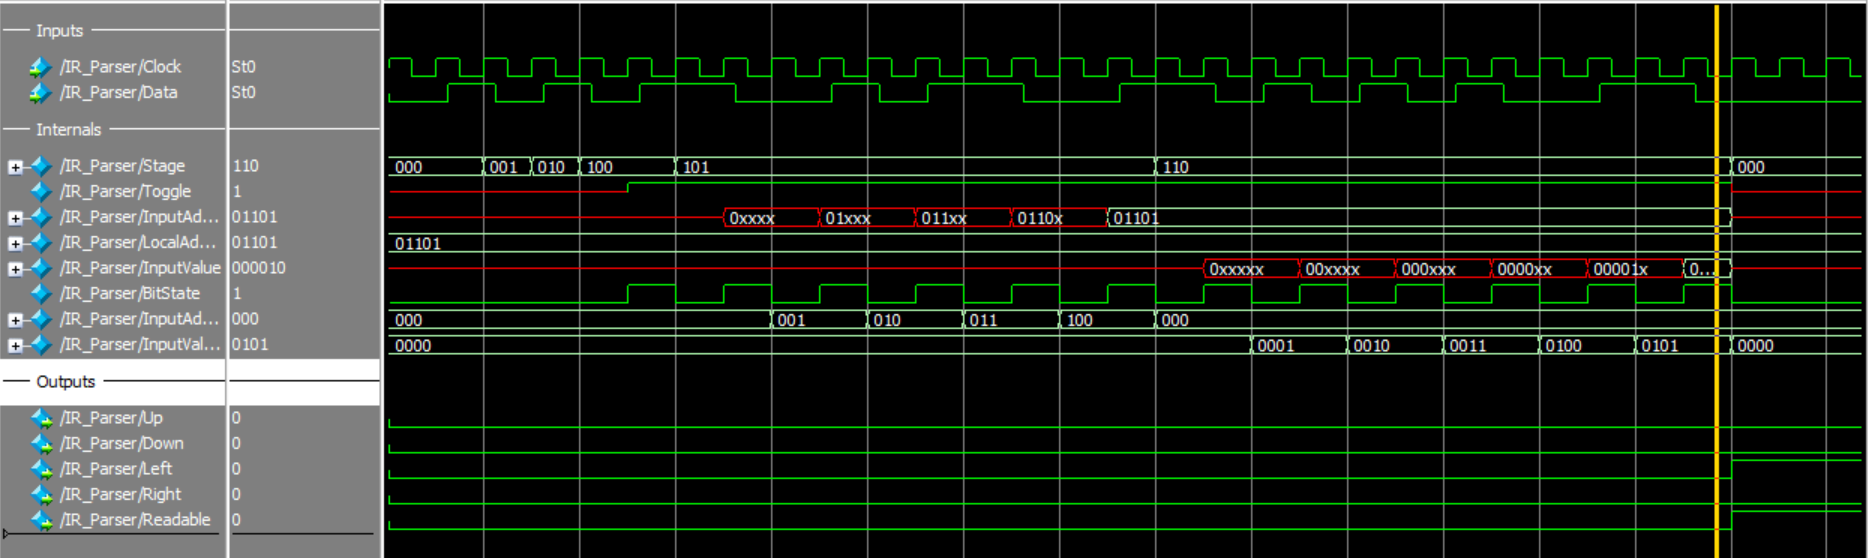
\includegraphics[width=\linewidth]{figures/IR_Parser_Sim.png}
    \caption{IR Decoder Simulation}
    \label{fig:irParserSim}
\end{figure}
\paragraph{Inputs:} TODO
\paragraph{Outputs:} TODO
\paragraph{Simulation:} TODO
\paragraph{Description:} TODO

\subsection{PS/2 Input Decoder}
\begin{figure}[H]\centering
    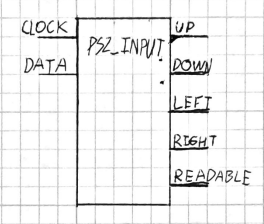
\includegraphics[width=0.5\linewidth]{figures/PS2_Input_Block.png}
    \caption{PS/2 Input Block}
    \label{fig:ps2InputBlock}
\end{figure}
\begin{figure}[H]\centering
    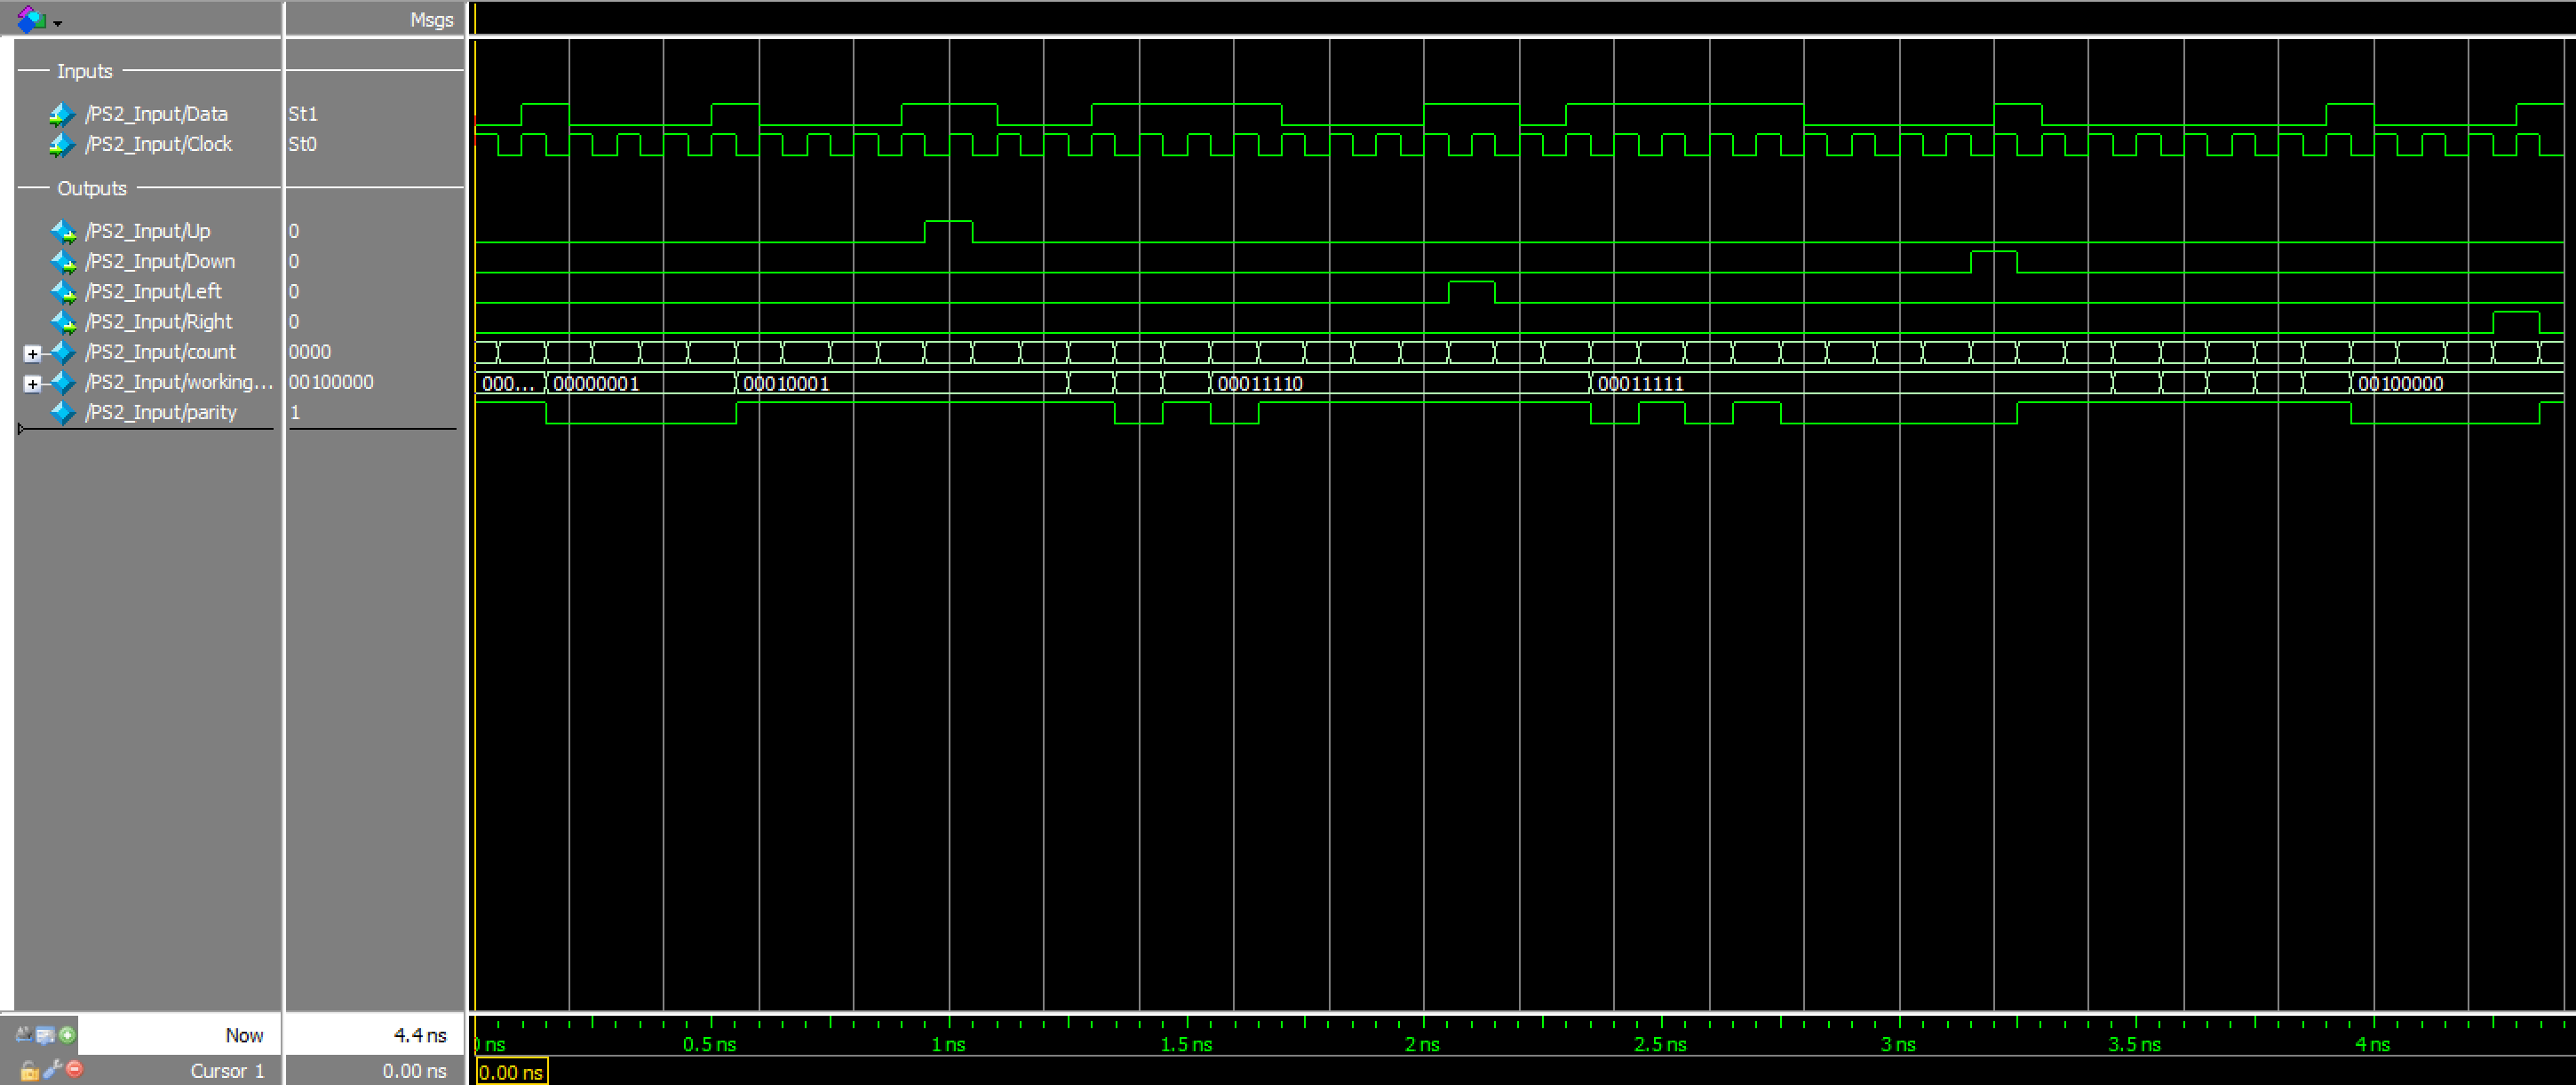
\includegraphics[width=\linewidth]{figures/PS2_Input_Sim.png}
    \caption{PS/2 Input Simulation}
    \label{fig:ps2ParserSim}
\end{figure}
\paragraph{Inputs:} There are two inputs for this module, the CLK and Data signal from the PS/2 Port.
\paragraph{Outputs:} One output for each cardinal direction (Up, Down, Left, Right), and signal describing whether or not the directions are valid or not, 'Readable'.
\paragraph{Simulation:} This simulation feeds valid PS/2 inputs that represent the keys W, A, S, and D being pressed down, which should result in the output of Up, Left, Down, then Right.
\paragraph{Description:} This module essentially functions as a shift register, with some extra logic to handle the PS/2 standard.  It waits for the 2nd bit, and reads each bit from 2 through 9 into a data register, starting with the least significant bit and ending with the most significant bit.  In addition to storing the data, every time a 1 is received it updates an internal parity bit.  The 10th bit is the keyboard's parity bit, and is compared to the internally tracked parity bit.  If they match, it updates the outputs to indicate which key was pressed, depending on which data was transferred.  If the parity bits don't match, nothing occurs.  When the 11th bit is transferred, everything is reset to its initial state.

\subsection{Input Decoder/Multiplexer}
\begin{figure}[H]\centering
    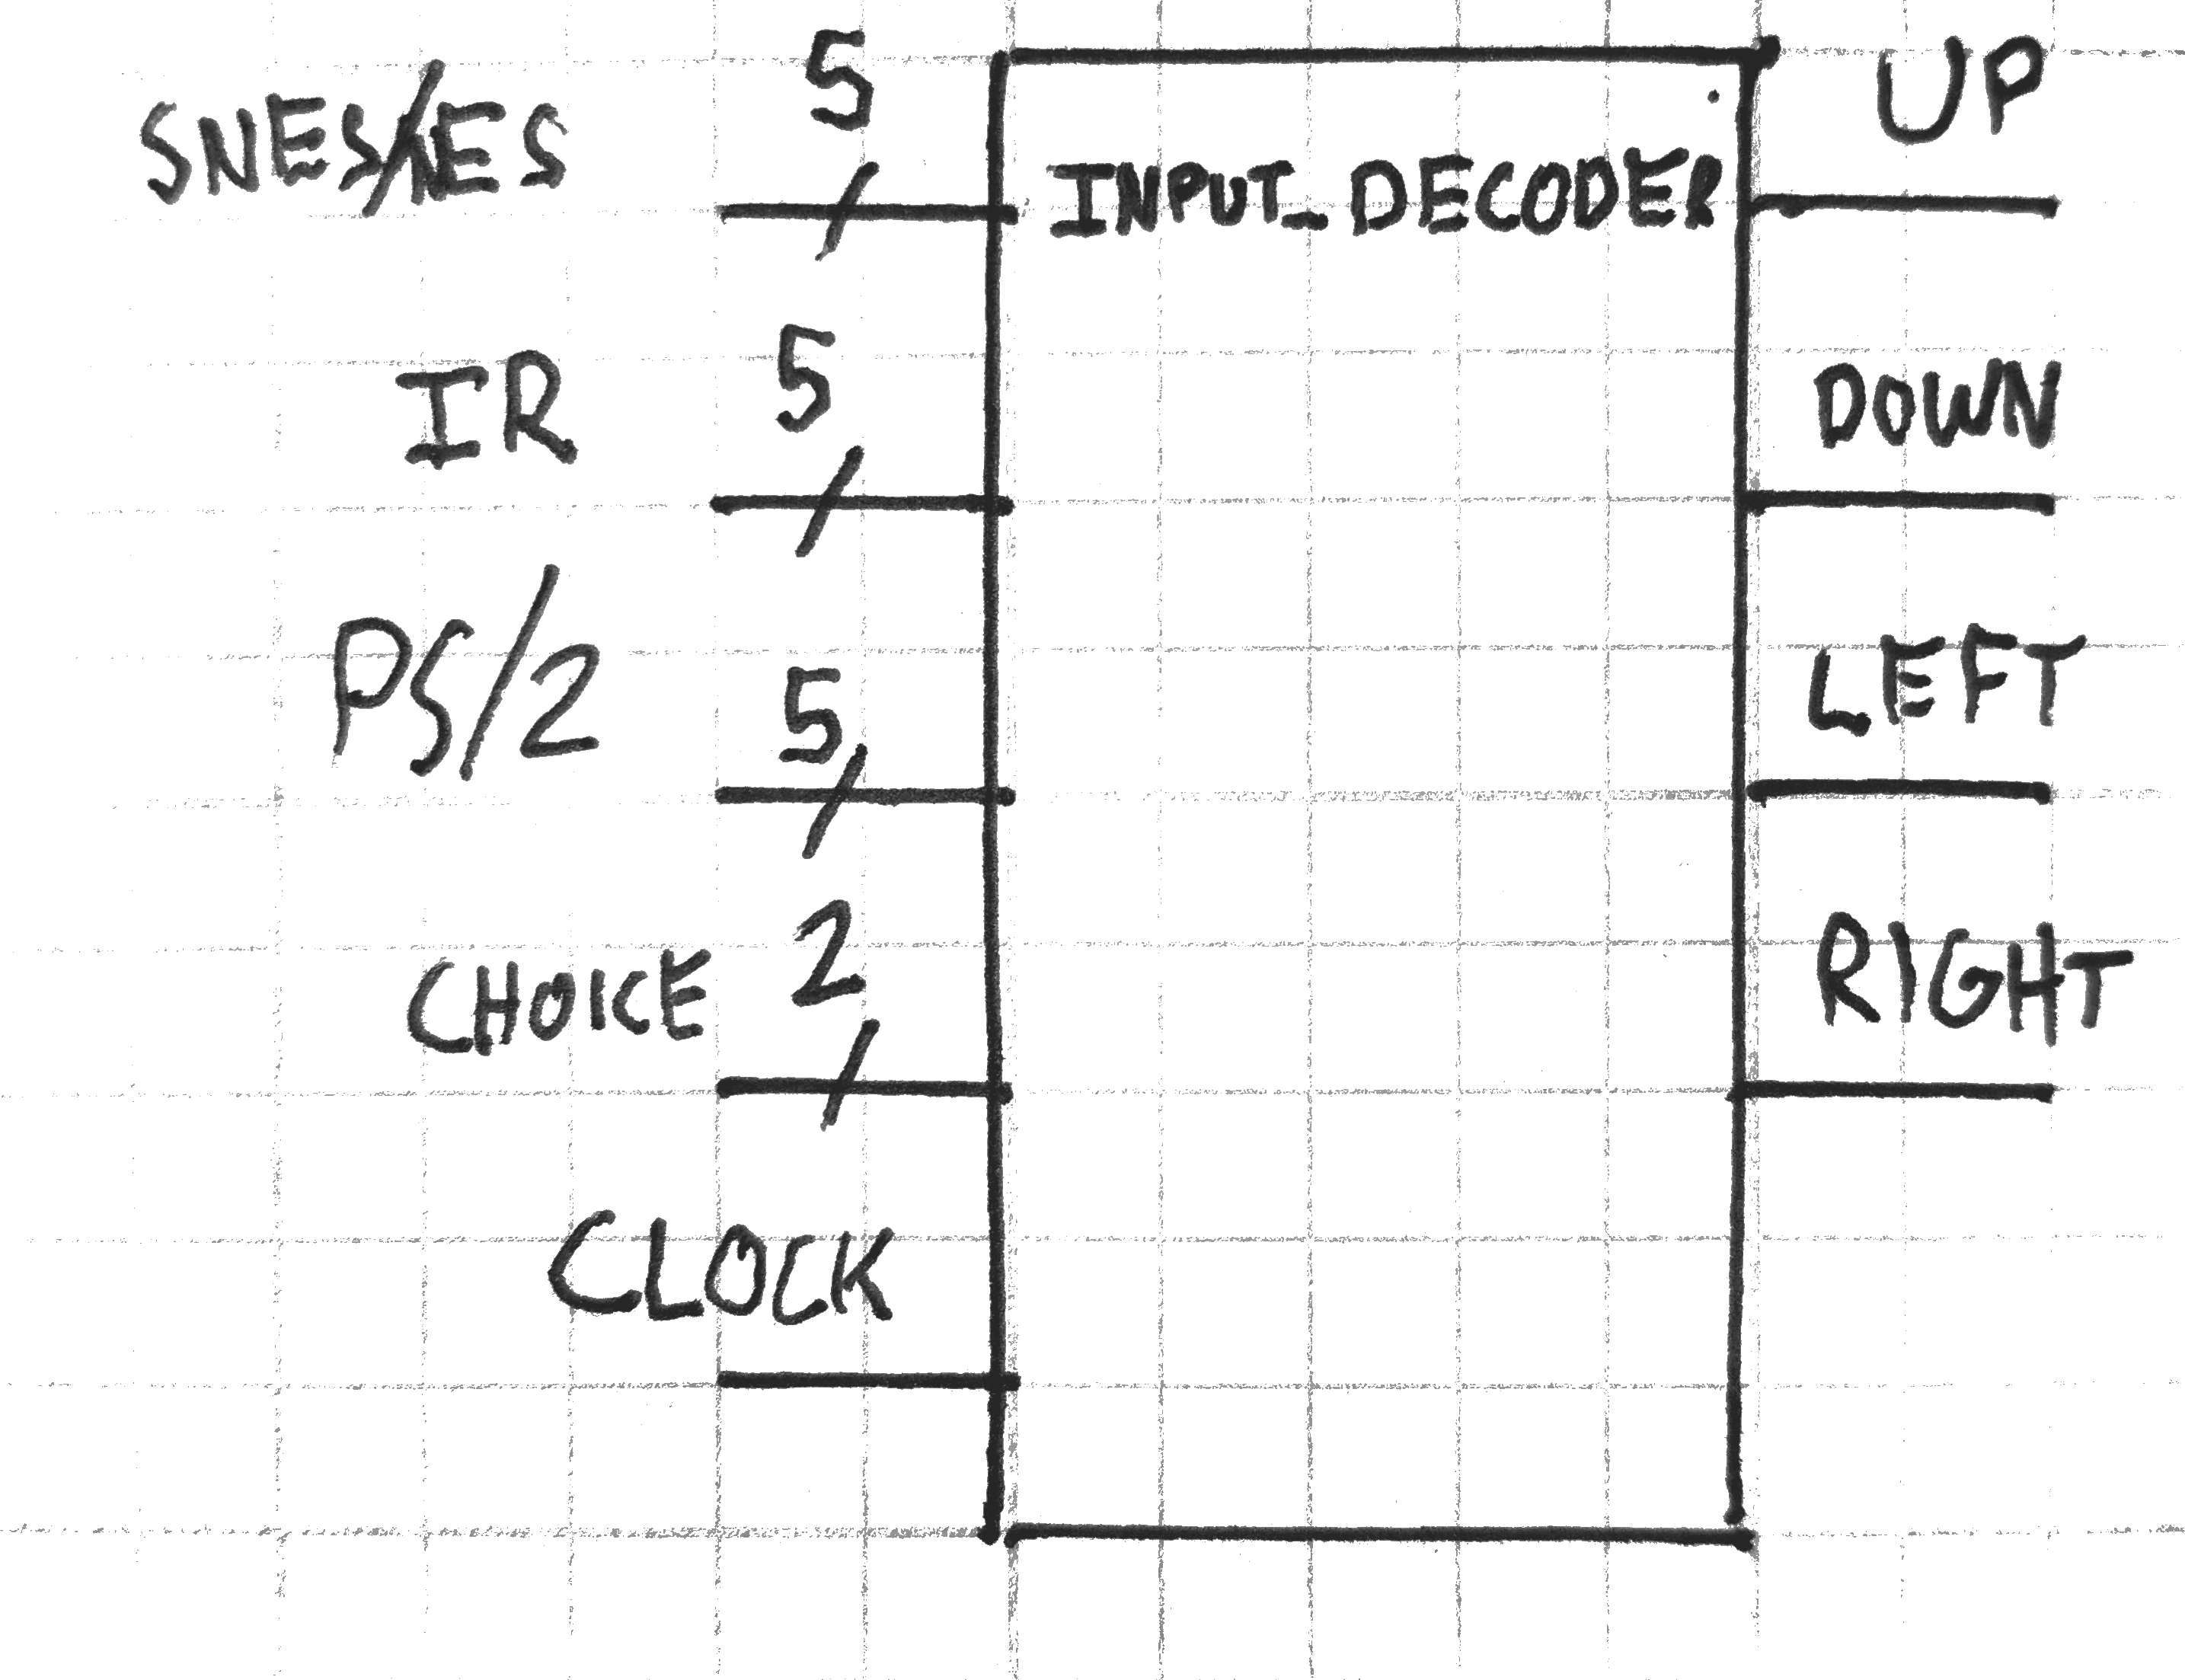
\includegraphics[width=0.5\linewidth]{figures/Input_Decoder_Block.jpg}
    \caption{Input Decoder Block Diagram}
    \label{fig:inputDecoderBlock}
\end{figure}
\begin{figure}[H]\centering
    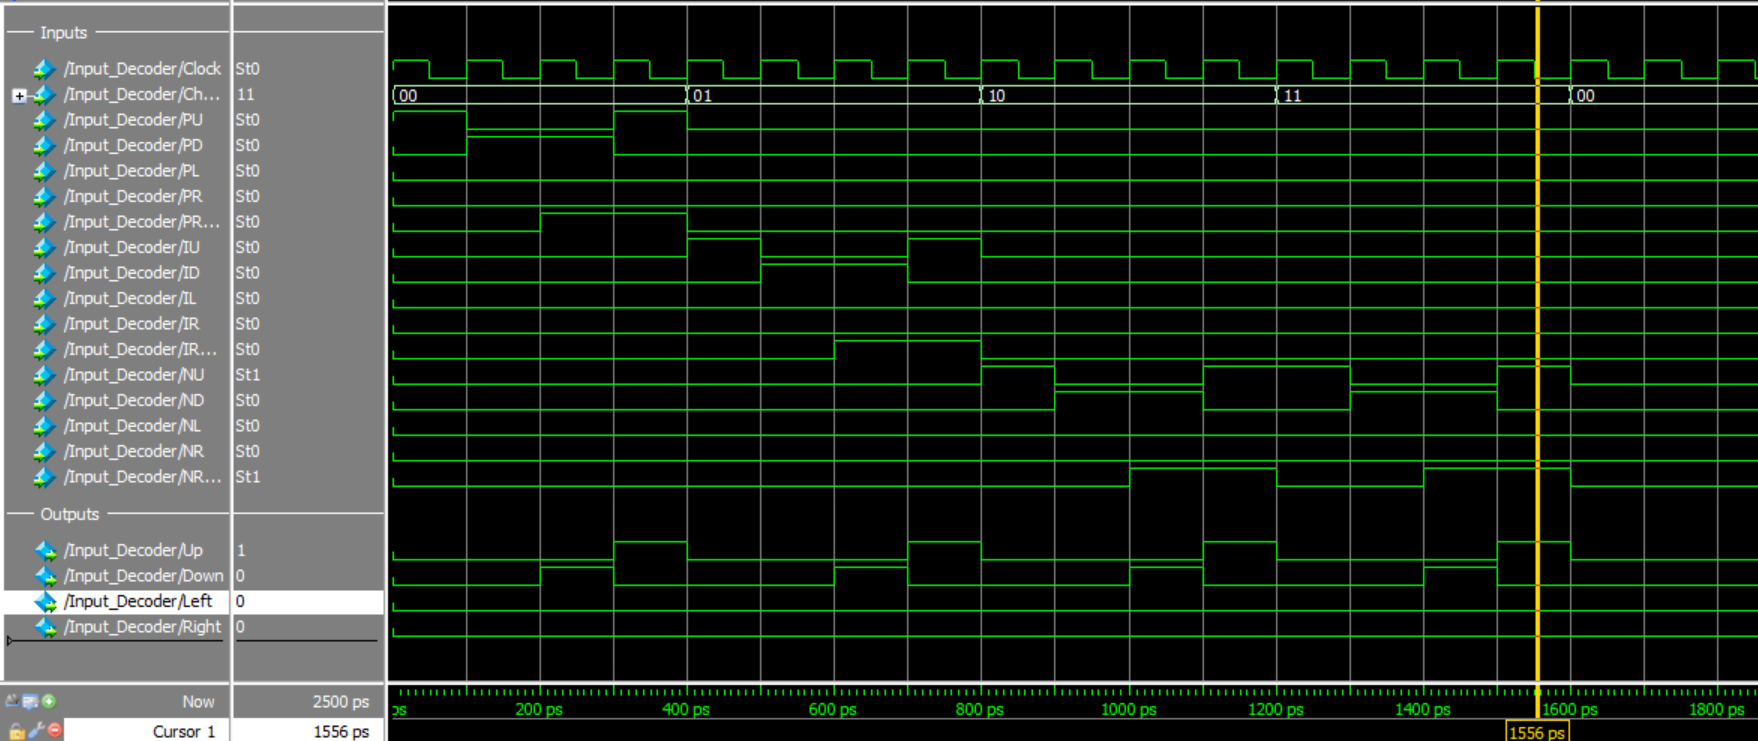
\includegraphics[width=0.5\linewidth]{figures/Input_Decoder_Sim.png}
    \caption{Input Decoder Simulation}
    \label{fig:inputDecoderSum}
\end{figure}
\paragraph{Inputs:} TODO
\paragraph{Outputs:} TODO
\paragraph{Simulation:} TODO
\paragraph{Description:} TODO

\subsection{Game Logic Controller}
\begin{figure}[H]\centering
	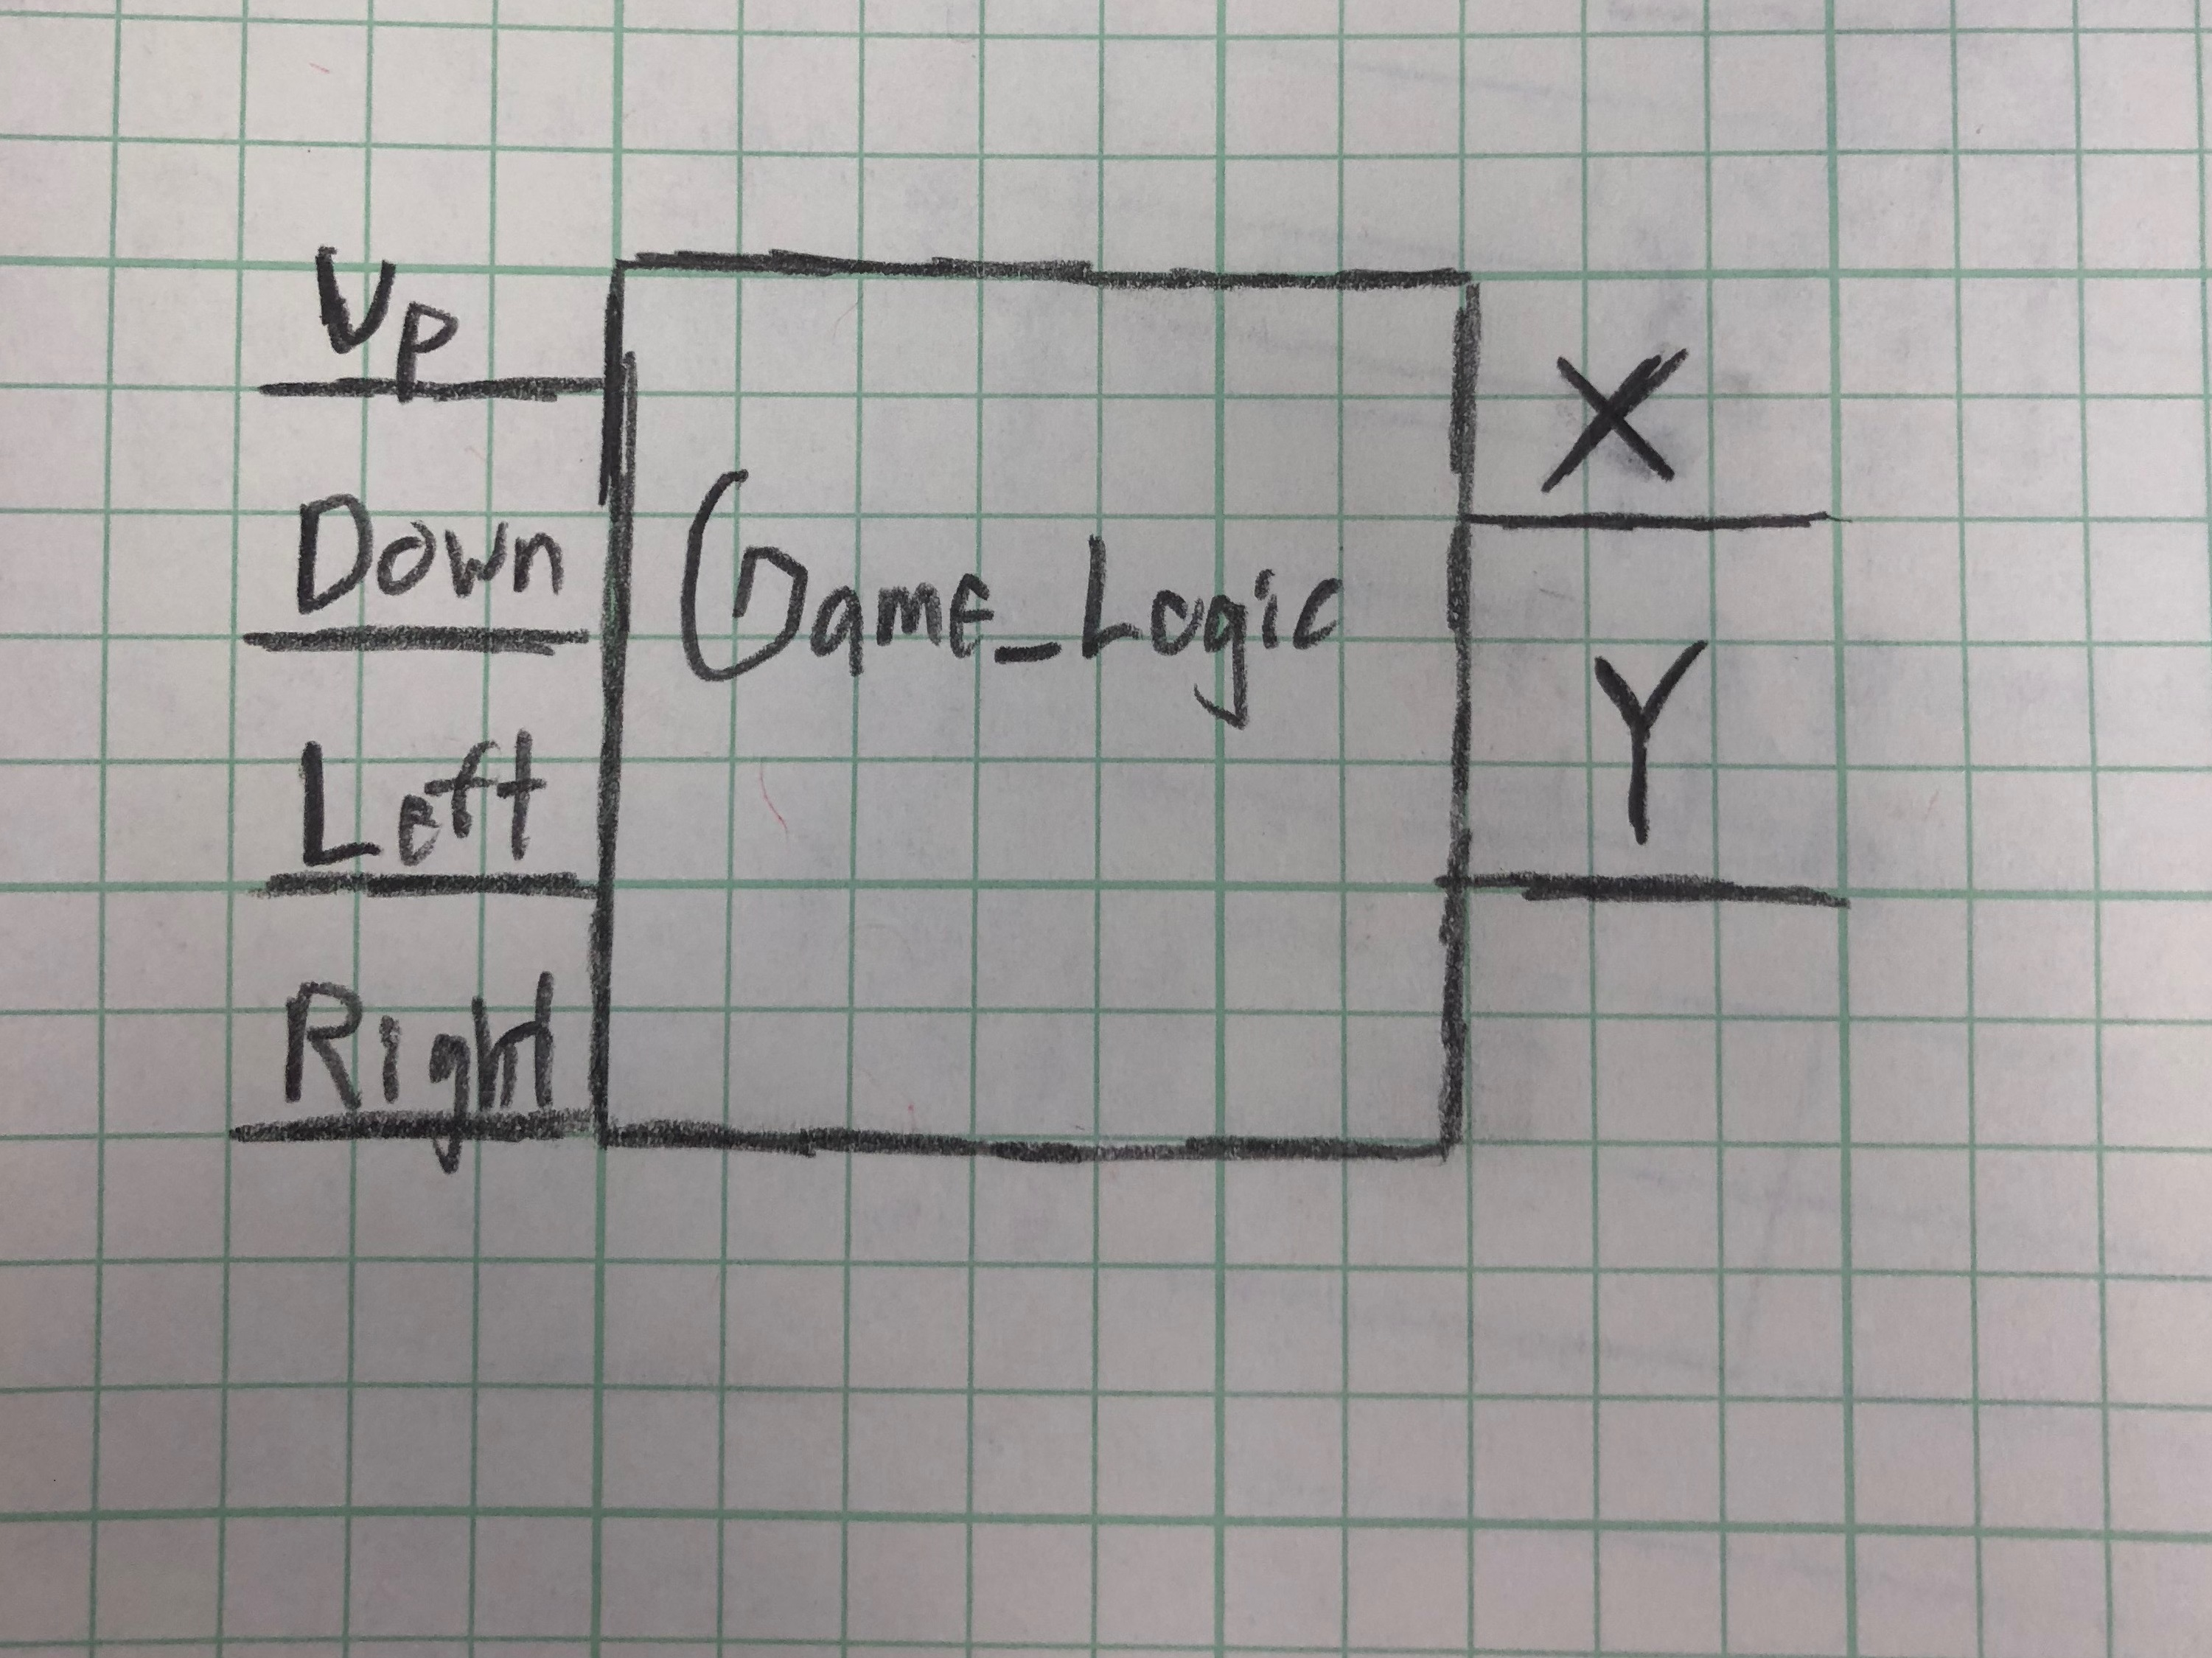
\includegraphics[width=\linewidth]{figures/Game_Logic_Diagram}
	\caption{Block Diagram of the Game Logic Controller}
\end{figure}
\begin{figure}[H]\centering
	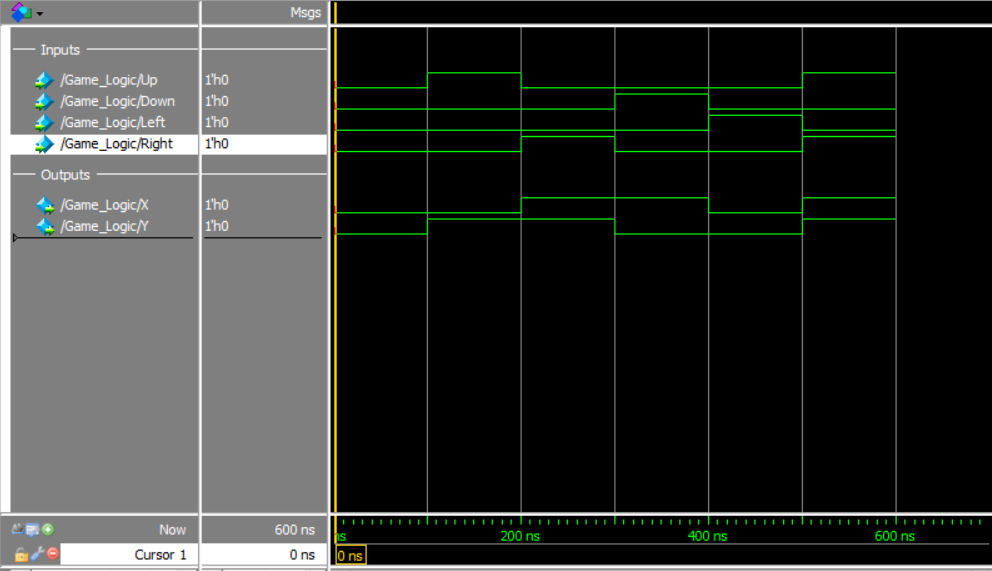
\includegraphics[width=\linewidth]{figures/Game_Logic_ModelSim.png}
	\caption{ModelSim of the Game Logic Controller.}
\end{figure}
\paragraph{Inputs:} One bit inputs for up, down, left, and right
\paragraph{Outputs:} One bit data inputs for X and Y, representing the position of the player object within the four by four grid where 0,0 is the lower left corner.
\paragraph{Simulation:} Within this simulation, the initial position of the player, 0,0. The up input is driven high, and as expected the coordinate output for Y also changes to high. Next, a right input is provided, and again the coordinates change such that X is high. After this, down is driven high and then left is driven high, resulting in the coordinates shifting to 0,1 then 0,0. Finally, both up and right are driven high, resulting in a coordinate of 1,1.
\paragraph{Description:} This module will use combinational logic to determine the coordinate state of a player. The current position is stored within the module, and from the provided values of up, down, left, and right the next position is determined. An input that would result in the player going outside of the coordinate bounds(0,0 to 1,1) is ignored. Multiple inputs can be accepted at once, allowing for diagonal movement.

\subsection{Player Top Module}
\begin{figure}[H]\centering
    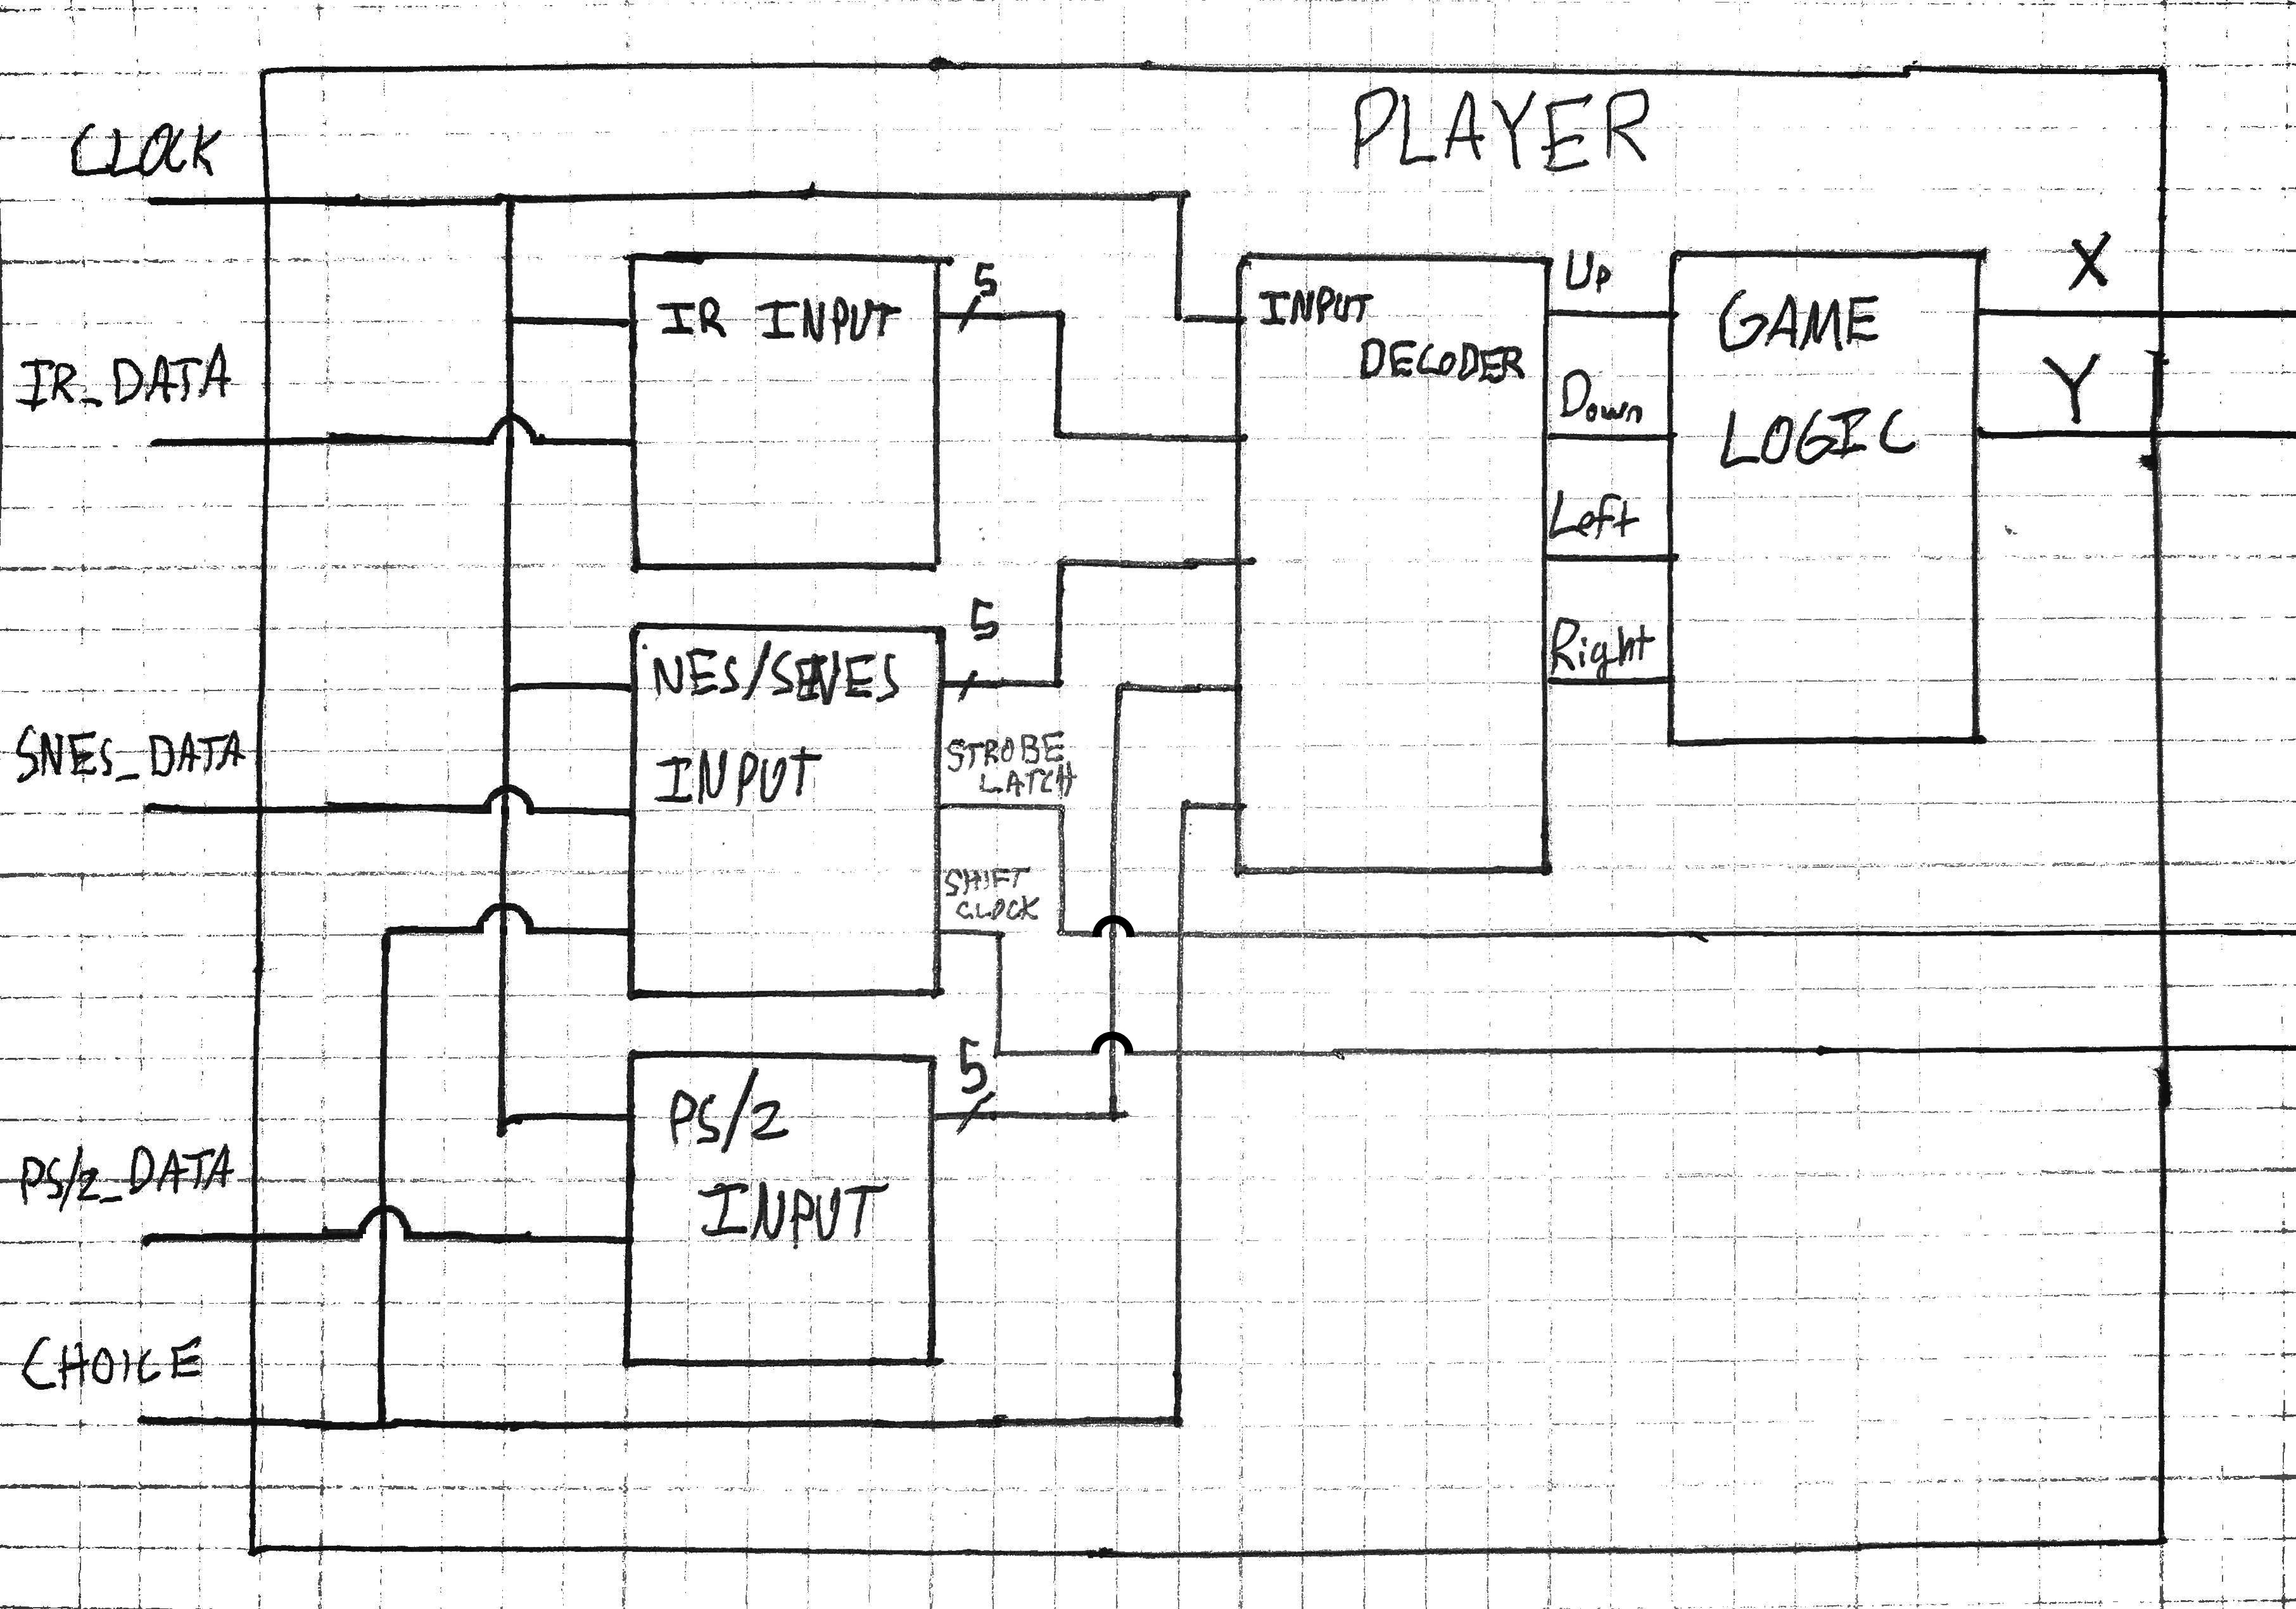
\includegraphics[width=\linewidth]{figures/Player_Block.jpg}
    \caption{Player Block Diagram}
    \label{fig:playerBlock}
\end{figure}
\begin{figure}[H]\centering
    
\includegraphics[width=0.5\linewidth]{figures/placeholder.png}
    \caption{Player Simulation}
    \label{fig:playerSim}
\end{figure}
\paragraph{Inputs:} TODO
\paragraph{Outputs:} TODO
\paragraph{Simulation:} TODO
\paragraph{Description:} TODO

\subsection{Pixel Counter}
\begin{figure}[H]\centering
    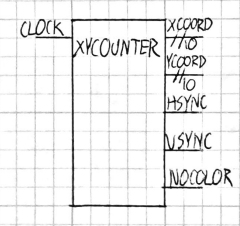
\includegraphics[width=0.5\linewidth]{figures/XYCounter_Block.png}
    \caption{Pixel Counter Block}
    \label{fig:pixelCounterBlock}
\end{figure}
\begin{figure}[H]\centering
    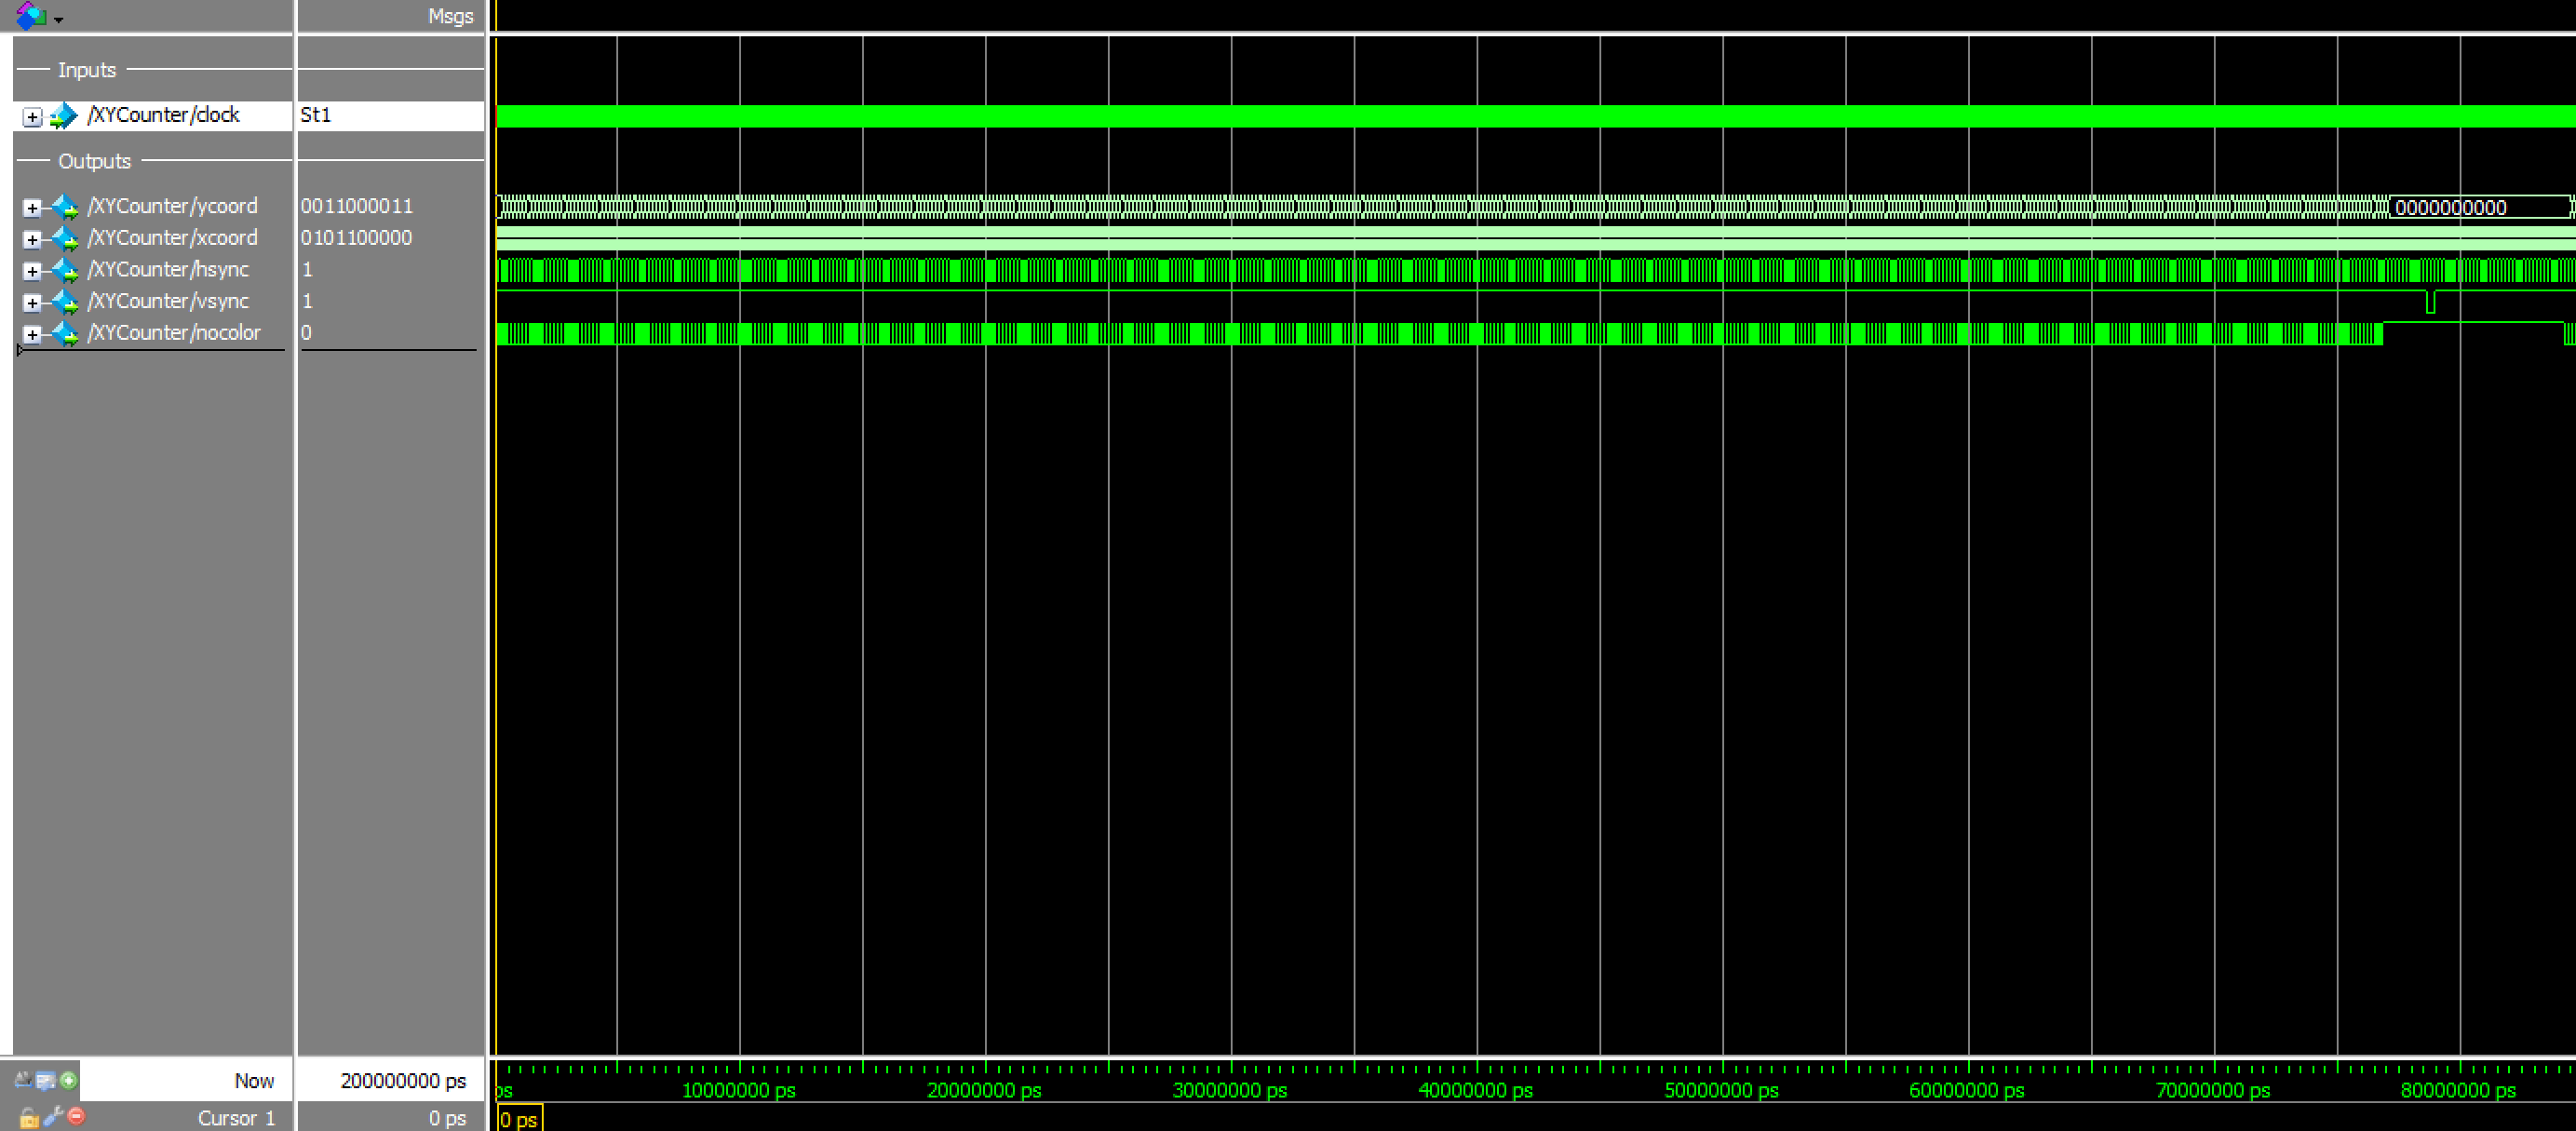
\includegraphics[width=\linewidth]{figures/XYCounter_Sim_Frame.png}
    \caption{Pixel Counter Simulation Frame-Scale}
    \label{fig:pixelCounterSimFrame}
\end{figure}
\begin{figure}[H]\centering
    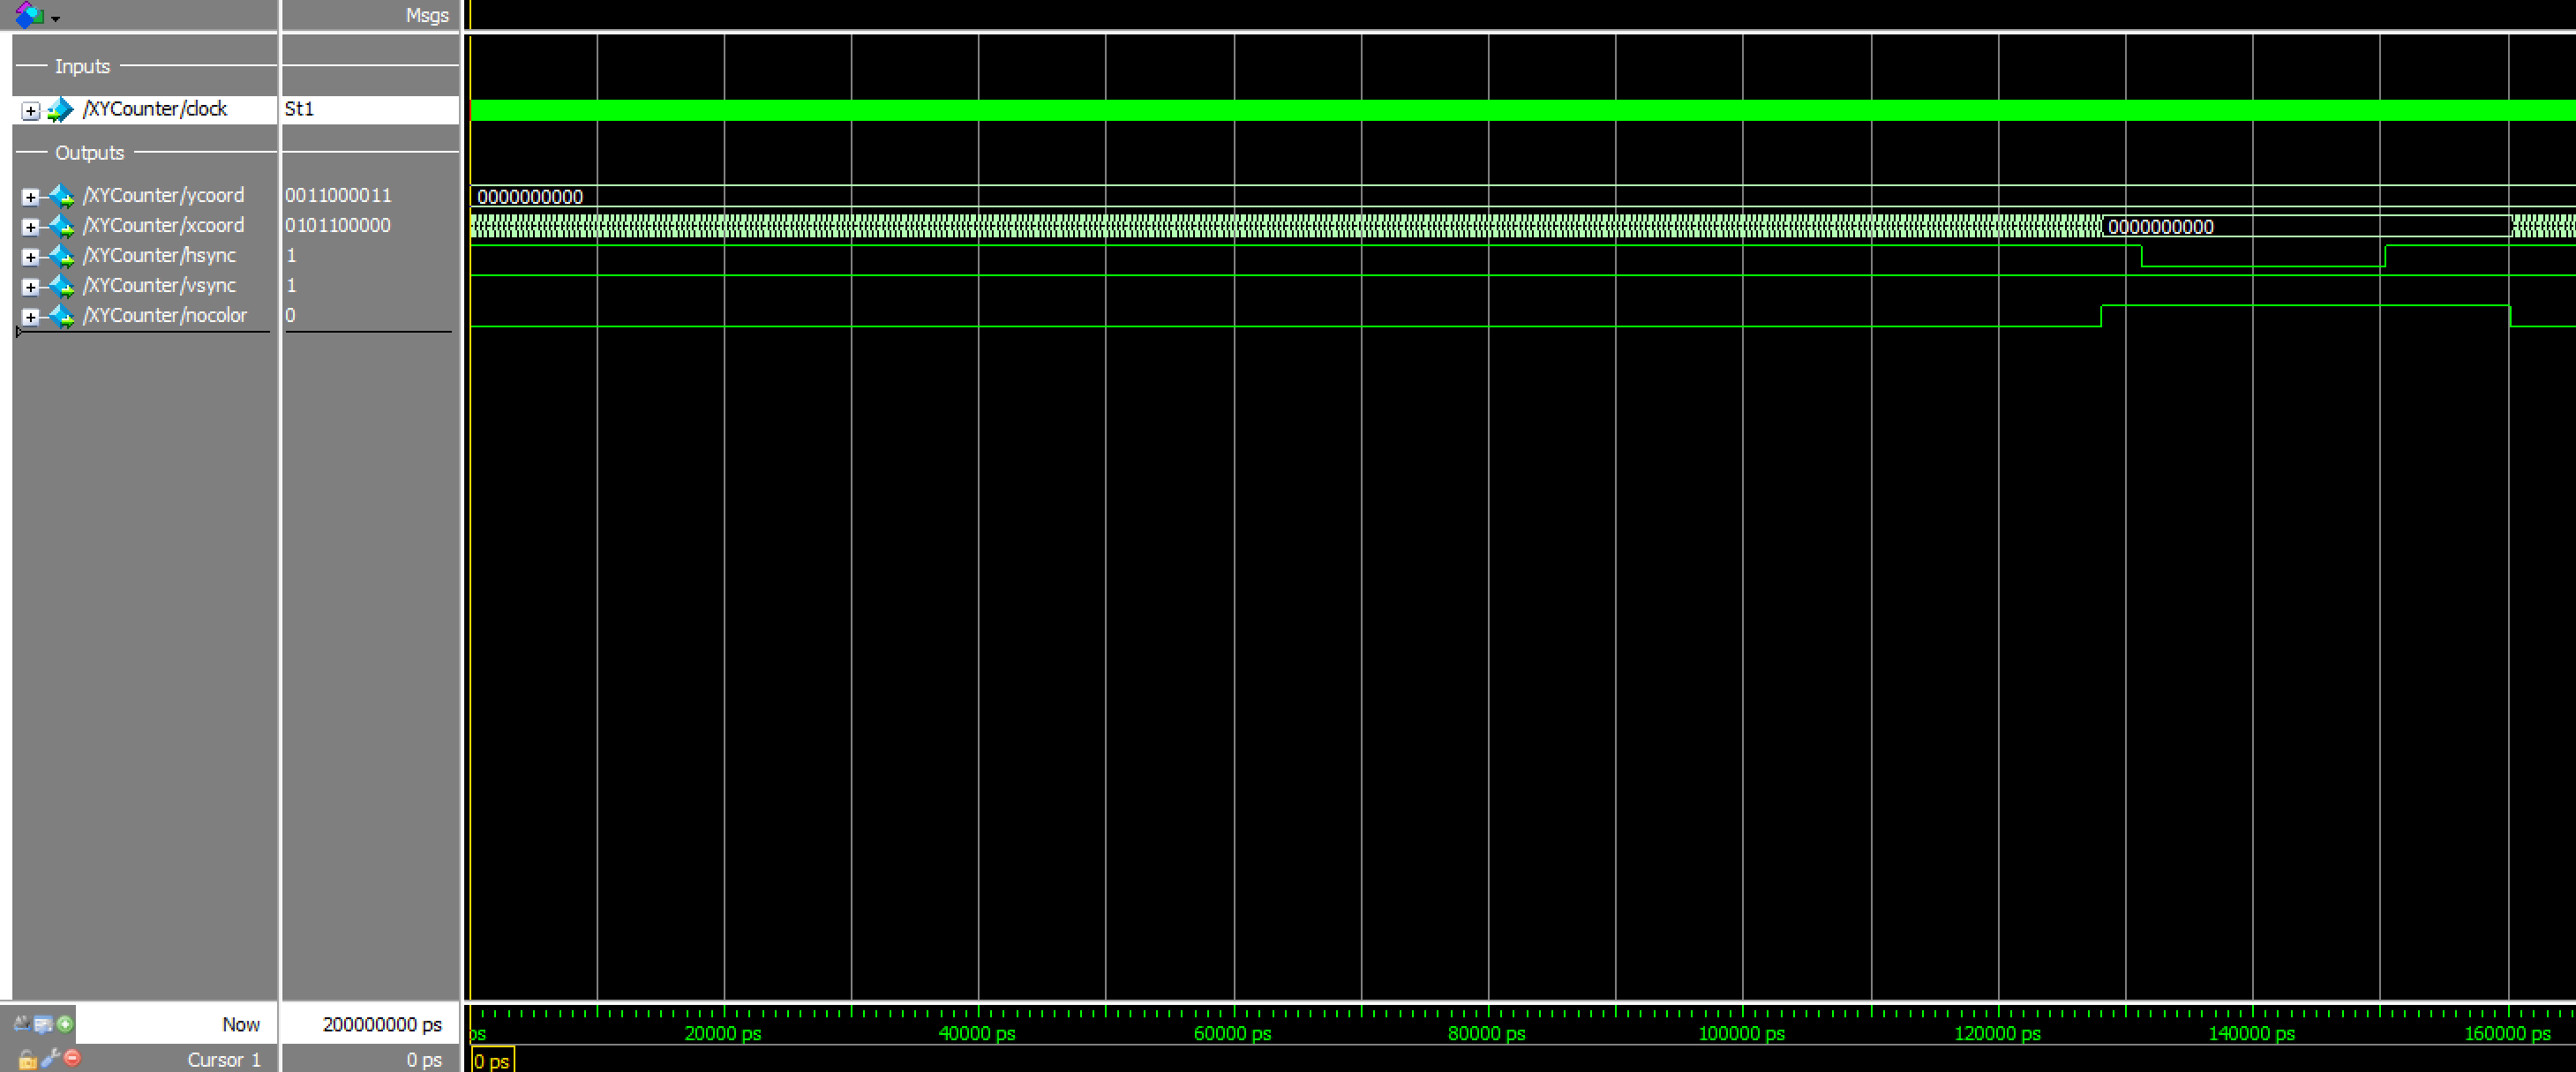
\includegraphics[width=\linewidth]{figures/XYCounter_Sim_Line.png}
    \caption{Pixel Counter Simulation Line-Scale}
    \label{fig:pixelCounterSimLine}
\end{figure}
\begin{figure}[H]\centering
    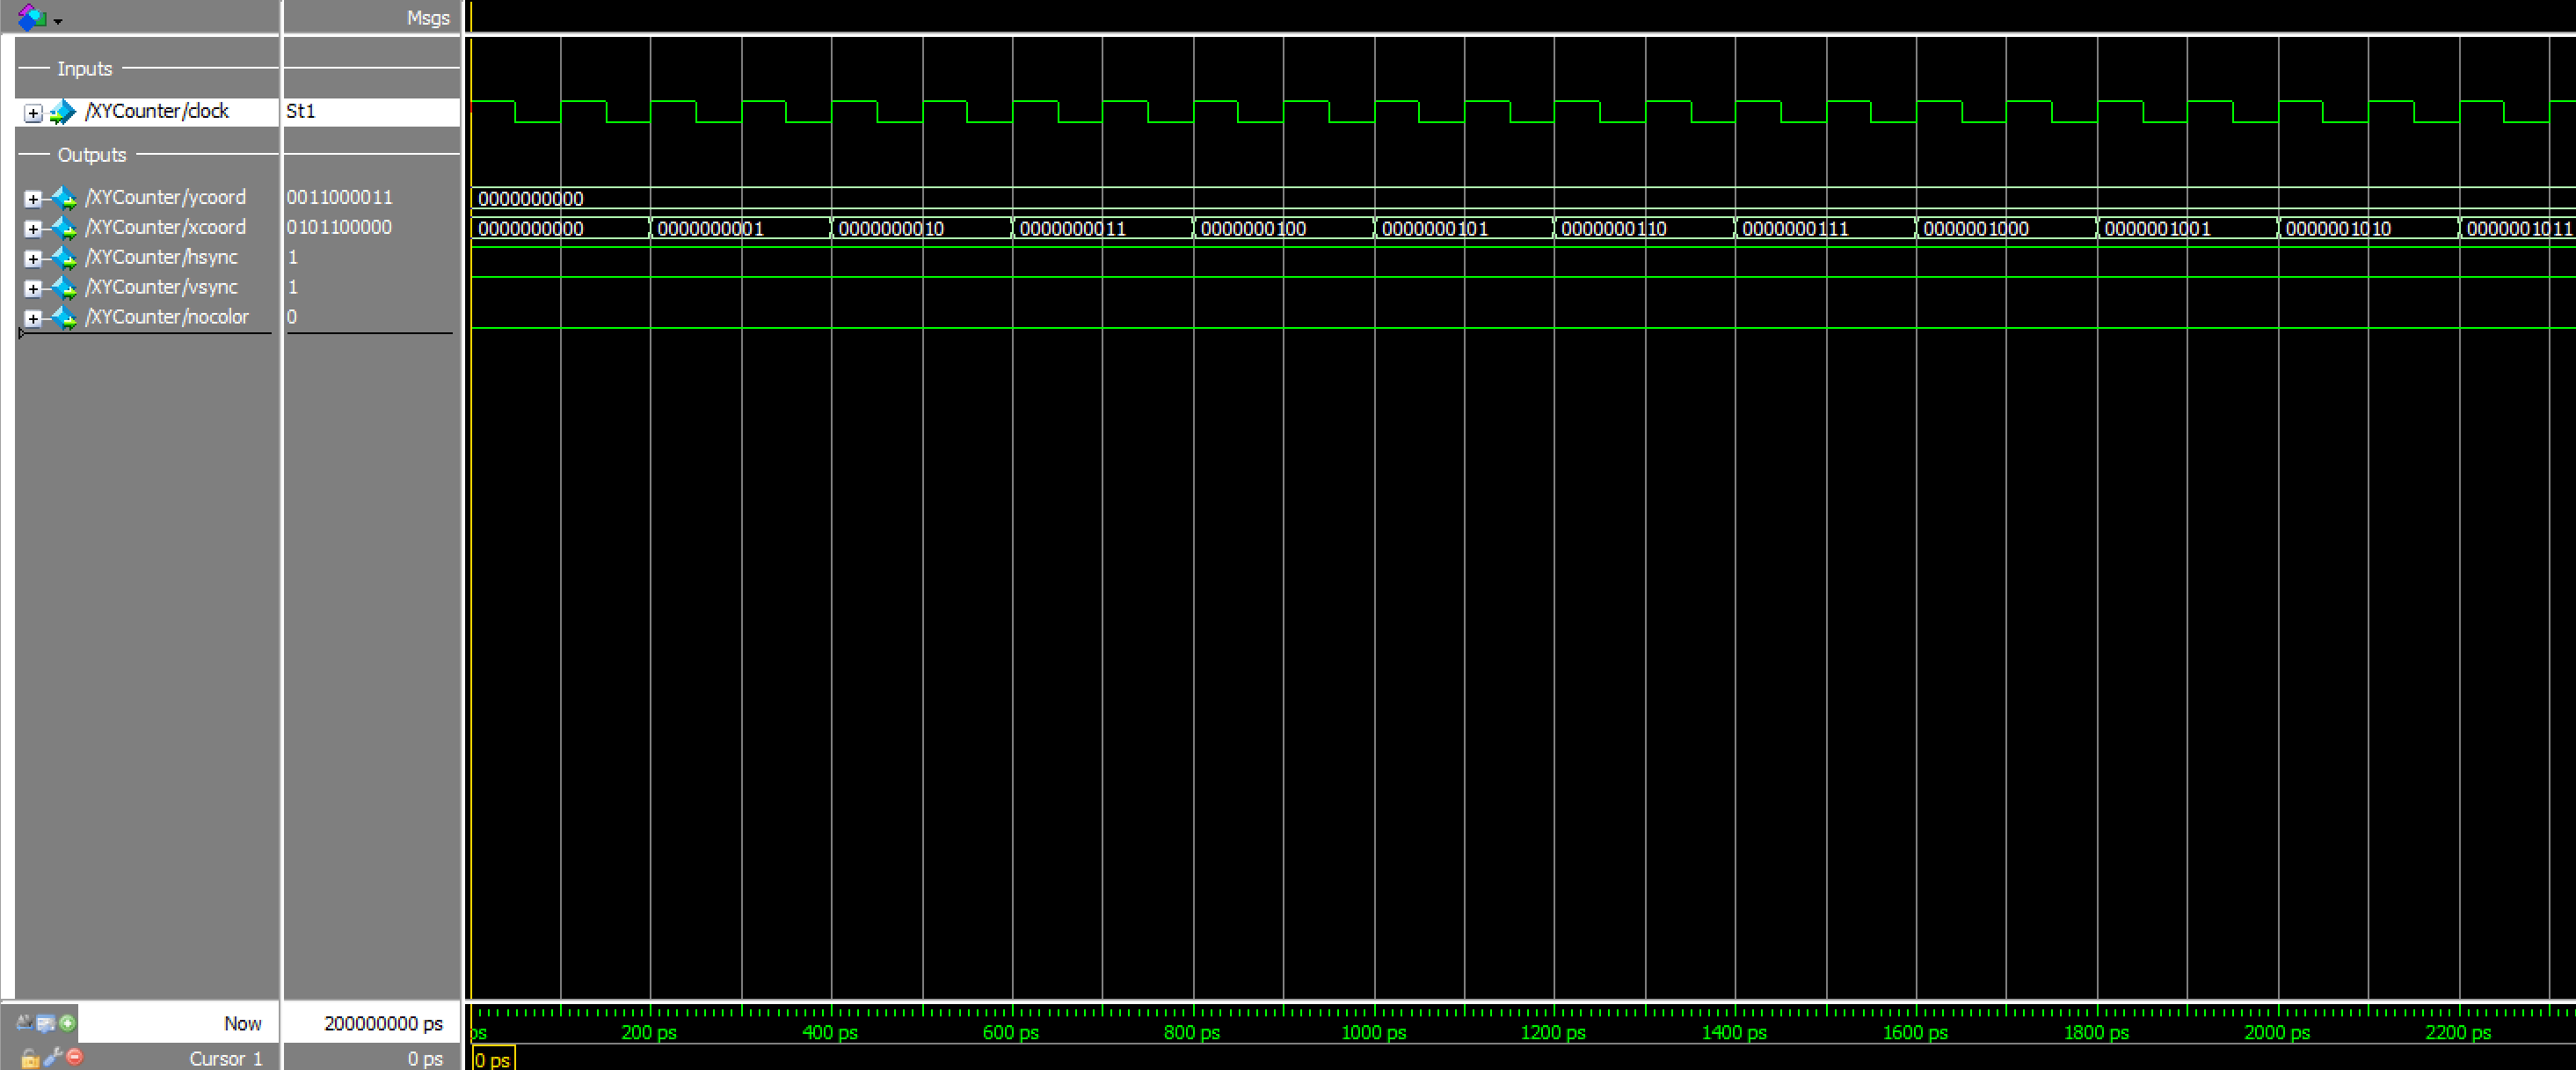
\includegraphics[width=\linewidth]{figures/XYCounter_Sim_Pixels.png}
    \caption{Pixel Counter Simulation Pixel-Scale}
    \label{fig:pixelCounterSimPixels}
\end{figure}
\paragraph{Inputs:} A 50MHz clock signal.
\paragraph{Outputs:} X and Y coordinates indicating the current pixel being drawn on the monitor, an HSync and VSync signal that is fed directly to the VGA output, and a nocolor signal indicating when the color outputs on the VGA should be brought to 0.
\paragraph{Simulation:} In this simulation, the only input provided is that of a 50MHz clock signal.  The output is sampled for an entire second, and then the waves can be viewed to verify that the timing of all the outputs is correct.
\paragraph{Description:} Every clock pulse, a clock enable bit is flipped, and the logic is only updated when the clock enable is 1.  There are two internal registers, xstate and ystate, which keep track of the current state in the current row and column.  It will drive nocolor to 1 when there should be no color output, and pulse HSync and VSync whenever they need to be pulsed, according to the timings for a 640 x 480 60Hz signal (described in Section \ref{vidoutput}).

\subsection{Renderer}
\begin{figure}[H]\centering
    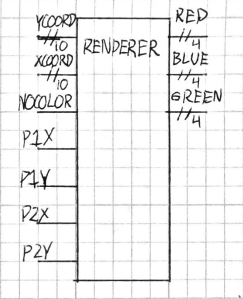
\includegraphics[width=0.5\linewidth]{figures/Renderer_Block.png}
    \caption{Renderer Block}
    \label{fig:rendererBlock}
\end{figure}
\begin{figure}[H]\centering
    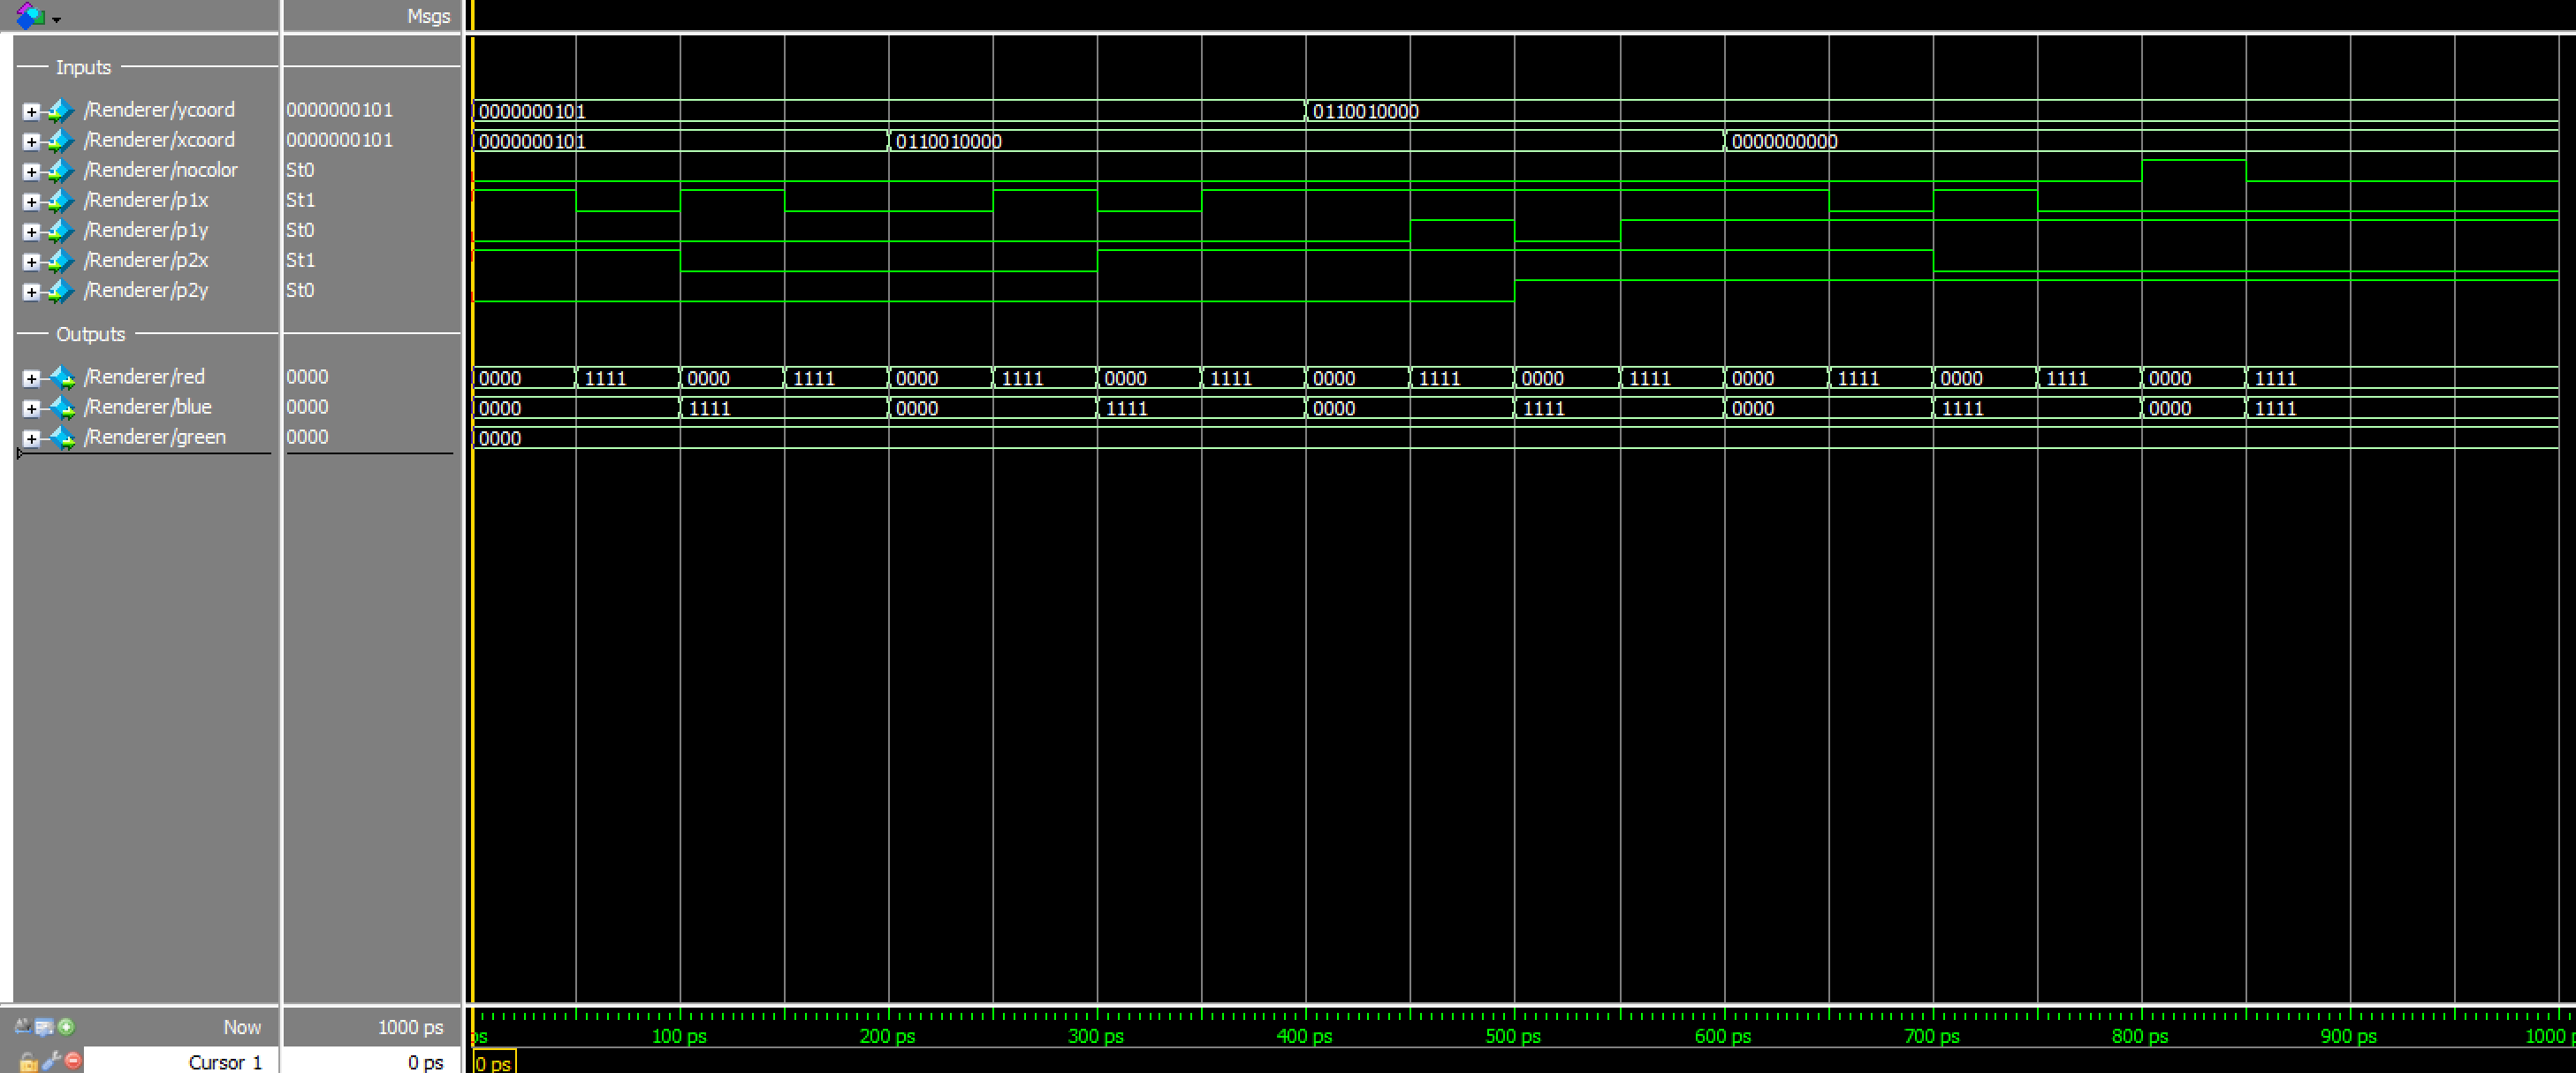
\includegraphics[width=\linewidth]{figures/Renderer_Sim.png}
    \caption{Renderer Simulation}
    \label{fig:rendererSim}
\end{figure}
\paragraph{Inputs:} 4 bits that indicate the x and y coordinate of both players, a nocolor signal indicating when the Renderer needs to output low for all colors as part of VGA timings, and the x and y coordinate of the current pixel being drawn by VGA.
\paragraph{Outputs:} The Red, Green, and Blue values for the current pixel being rendered, represented as three four bit values. 
\paragraph{Simulation:} In this simulation, it drives the x and y inputs to 4 coordinates, one in each quadrant.  For each coordinate, it drives the player locations of each player such that it tests the four possible color states for each coordinate: no players in quadrant, player 1 in quadrant, player 2 in quadrant, both players in quadrant.  Finally, it drives nocolor to 1, to test that color output is set to 0 when nocolor is 1.
\paragraph{Description:} If the nocolor input is 1, all color outputs are driven to 0.  Next, it will immediately drive green to 0 as it's not used in our display.  Next, it will check what quadrant of the screen the current pixel being drawn is in, and what players are located in that quadrant.  If player 1 is in the quadrant, red is driven to full color, otherwise it's driven to 0.  Same for player 2 and blue.

\section{Putting it Together}
TODO

\section{Extra Implementation}
TODO
\section{Appendix}
TODO

\begin{thebibliography}{99}
    \bibitem{vishayIr}
    Vishay. Data Formats for IR Remote Control. 
    \\\texttt{https://www.vishay.com/docs/80071/dataform.pdf}
\end{thebibliography}

\end{document}